\clearpage
\begin{appendices}

%Some Table of Contents entry formatting
\addtocontents{toc}{\protect\renewcommand{\protect\cftchappresnum}{\appendixname\space}}
\addtocontents{toc}{\protect\renewcommand{\protect\cftchapnumwidth}{6em}}

%Begin individual appendices, separated as chapters

\chapter{Default Detection and Discrimination}

% Detection/Discrimination each dataset
% PETS1
\begin{sidewaystable}
\centering
\caption{PETS1 - Detection ($\eta$) and Discrimination ($\xi$) for each shadow removal method (default parameters)}
%\caption*{Detection ($\eta$) and Discrimination ($\xi$) for each shadow removal method (default parameters)}
\begin{tabular}{ |c|c|c|c|c|c|c|c|c|c|c| }
	\hline
\textbf{frame} &  \textbf{C - $\eta$} &  \textbf{C - $\xi$} &  \textbf{P - $\eta$} &  \textbf{P - $\xi$} &  \textbf{G - $\eta$} &  \textbf{G - $\xi$} &  \textbf{SRT - $\eta$} &  \textbf{SRT - $\xi$} &  \textbf{LRT - $\eta$} &  \textbf{LRT - $\xi$} \\
\hline
\hline
44 & 82.3629 &  75.7402 &   69.2827 &  75.9517 &   76.8776 &  91.0876 &   14.0084 &  92.9003 &   32.6582 &  98.4592 \\
\hline
49 & 67.6524 &  70.5788 &   53.1080 &  83.4889 &   80.9897 &  91.5978 &   3.3796 &  99.7866 &   11.5269 &  100.0000 \\
\hline
67 & 77.9240 &  67.8265 &   65.6433 &  67.6909 &   90.3509 &  89.2454 &   8.3333 &  90.8269 &   0.0000 &  96.2494 \\
\hline
73 & 98.0328 &  61.8231 &   66.2295 &  64.7059 &   66.2295 &  52.2400 &   25.2459 &  81.3011 &   0.0000 &  97.4289 \\
\hline
77 & 72.4427 &  69.9954 &   79.6947 &  76.0390 &   61.6031 &  82.1130 &   5.4198 &  97.5186 &   57.9389 &  94.1848 \\
\hline
82 & 75.2788 &  69.7977 &   78.6989 &  73.8816 &   75.7993 &  59.8849 &   39.7026 &  82.6434 &   50.3346 &  93.9391 \\
\hline
85 & 71.4528 &  63.2595 &   68.8791 &  66.9706 &   63.0545 &  59.8664 &   84.1856 &  50.4082 &   32.3061 &  95.5784 \\
\hline
91 & 84.2899 &  64.9629 &   71.5467 &  68.4584 &   64.3482 &  89.5301 &   32.9280 &  87.0404 &   30.7393 &  87.0899 \\
\hline
107 & 25.1656 &  83.2055 &   63.1347 &  80.6748 &   51.8764 &  97.3160 &   52.3179 &  81.8252 &   0.0000 &  100.0000 \\
\hline
124 & 28.0528 &  78.8076 &   79.3729 &  66.0321 &   65.8416 &  95.2405 &   17.3267 &  81.9639 &   45.3795 &  78.7074 \\
\hline
139 & 93.5268 &  60.4111 &   89.7321 &  57.1618 &   94.1964 &  91.1141 &   2.9018 &  98.9390 &   52.4554 &  79.5756 \\
\hline
167 & 15.1067 &  89.4986 &   88.5057 &  80.3523 &   80.6240 &  91.6667 &   58.9491 &  85.9756 &   60.4269 &  80.6911 \\
\hline
\end{tabular}

\end{sidewaystable}

% PETS2
\begin{sidewaystable}
\centering
\caption{PETS2 - Detection ($\eta$) and Discrimination ($\xi$) for each shadow removal method (default parameters)}
%\caption*{Detection ($\eta$) and Discrimination ($\xi$) for each shadow removal method (default parameters)}
\begin{tabular}{ |c|c|c|c|c|c|c|c|c|c|c| }
	\hline
\textbf{frame} &  \textbf{C - $\eta$} &  \textbf{C - $\xi$} &  \textbf{P - $\eta$} &  \textbf{P - $\xi$} &  \textbf{G - $\eta$} &  \textbf{G - $\xi$} &  \textbf{SRT - $\eta$} &  \textbf{SRT - $\xi$} &  \textbf{LRT - $\eta$} &  \textbf{LRT - $\xi$} \\
\hline
\hline
00009 &  72.8181 &  78.0194 &   68.2878 &  52.6612 &   72.5516 &  94.5496 &   70.0866 &  76.5609 &   26.5823 &  100.0000 \\
\hline
00019 &  37.3047 &  75.5725 &   46.8750 &  67.0760 &   0.0000 &  100.0000 &   44.7266 &  78.2609 &   0.0000 &  93.7604 \\
\hline
00029 &  50.7905 &  63.9494 &   44.2688 &  66.8265 &   0.0000 &  100.0000 &   64.2292 &  84.9172 &   3.1621 &  84.0453 \\
\hline
00054 &  77.8761 &  69.7446 &   99.1150 &  66.1100 &   0.0000 &  100.0000 &   69.0265 &  94.9902 &   0.0000 &  100.0000 \\
\hline
00077 &  57.9767 &  77.3554 &   99.3515 &  68.5402 &   0.2594 &  34.0477 &   74.8379 &  91.9127 &   83.5279 &  89.1225 \\
\hline
00078 &  74.1440 &  77.3310 &   100.0000 &  63.8533 &   0.0000 &  100.0000 &   8.9728 &  99.0278 &   93.5065 &  96.9951 \\
\hline
00081 &  74.2164 &  75.8822 &   99.0900 &  56.3435 &   0.0000 &  94.7242 &   7.7856 &  96.6769 &   91.4055 &  76.2019 \\
\hline
00084 &  78.4682 &  75.8360 &   99.2052 &  53.9914 &   0.0000 &  100.0000 &   69.0751 &  83.8008 &   89.3064 &  90.3452 \\
\hline
00088 &  21.7105 &  70.8188 &   100.0000 &  58.9431 &   0.0000 &  83.7398 &   0.0000 &  100.0000 &   78.2895 &  78.7747 \\
\hline
00115 &  15.1329 &  56.5330 &   25.7669 &  61.8370 &   0.0000 &  100.0000 &   23.9264 &  85.4463 &   0.0000 &  100.0000 \\
\hline
00177 &  84.5038 &  66.9796 &   73.6506 &  63.6037 &   0.0000 &  100.0000 &   45.6761 &  95.9648 &   27.7423 &  85.6173 \\
\hline
\end{tabular}

\end{sidewaystable}

% aton_highway1
\begin{sidewaystable}
\centering
\caption{aton\_highway1 - Detection ($\eta$) and Discrimination ($\xi$) for each shadow removal method (default parameters)}
%\caption*{Detection ($\eta$) and Discrimination ($\xi$) for each shadow removal method (default parameters)}
\begin{tabular}{ |c|c|c|c|c|c|c|c|c|c|c| }
	\hline
\textbf{frame} &  \textbf{C - $\eta$} &  \textbf{C - $\xi$} &  \textbf{P - $\eta$} &  \textbf{P - $\xi$} &  \textbf{G - $\eta$} &  \textbf{G - $\xi$} &  \textbf{SRT - $\eta$} &  \textbf{SRT - $\xi$} &  \textbf{LRT - $\eta$} &  \textbf{LRT - $\xi$} \\
\hline
\hline
0045 &  75.4613 &  69.9373 &   75.5500 &  68.9675 &   79.0454 &  87.1192 &   27.7857 &  88.2145 &   83.5167 &  93.0405    \\
\hline
0065 &  87.0106 &  66.1312 &   67.1580 &  65.4284 &   63.5191 &  78.4137 &   0.2303 &  98.3936 &   68.5398 &  91.8340    \\
\hline
0085 &  75.3393 &  71.7385 &   73.1796 &  57.4586 &   68.6852 &  80.9808 &   4.9759 &  98.7355 &   77.4259 &  92.8961    \\
\hline
0105 &  89.2308 &  76.0680 &   82.7473 &  69.9272 &   60.4396 &  78.6650 &   1.0989 &  94.0777 &   84.0659 &  84.7087    \\
\hline
0125 &  77.3199 &  62.2002 &   69.1618 &  63.3436 &   61.4522 &  85.8059 &   24.3622 &  96.1517 &   80.2635 &  82.1528    \\
\hline
0145 &  78.5626 &  57.9551 &   72.2989 &  64.8861 &   51.7468 &  59.1013 &   16.8586 &  91.7851 &   81.8087 &  89.3398    \\
\hline
0165 &  75.0502 &  73.0680 &   67.2983 &  63.0572 &   68.1883 &  64.7848 &   15.9345 &  94.7709 &   74.6483 &  90.2977    \\
\hline
0185 &  70.3516 &  69.2308 &   65.7503 &  67.0521 &   71.5381 &  75.5757 &   15.4536 &  93.6742 &   72.9706 &  91.1992    \\
\hline
\end{tabular}

\end{sidewaystable}

% aton_highway3
\begin{sidewaystable}
\centering
\caption{aton\_highway3 - Detection ($\eta$) and Discrimination ($\xi$) for each shadow removal method (default parameters)}
%\caption*{Detection ($\eta$) and Discrimination ($\xi$) for each shadow removal method (default parameters)}
\begin{tabular}{ |c|c|c|c|c|c|c|c|c|c|c| }
	\hline
\textbf{frame} &  \textbf{C - $\eta$} &  \textbf{C - $\xi$} &  \textbf{P - $\eta$} &  \textbf{P - $\xi$} &  \textbf{G - $\eta$} &  \textbf{G - $\xi$} &  \textbf{SRT - $\eta$} &  \textbf{SRT - $\xi$} &  \textbf{LRT - $\eta$} &  \textbf{LRT - $\xi$} \\
\hline
\hline
0101 &  76.2500 &  53.0201 &   79.3750 &  24.1611 &   38.7500 &  95.3020 &   1.8750 &  95.5257 &   21.2500 &  80.3132    \\
\hline
0201 &  62.7848 &  57.9273 &   74.9367 &  31.5545 &   46.3291 &  92.7301 &   0.0000 &  90.6419 &   45.0633 &  89.2498    \\
\hline
0301 &  84.8361 &  55.9625 &   75.4098 &  35.4344 &   10.6557 &  98.0409 &   13.9344 &  81.6865 &   0.0000 &  98.0409    \\
\hline
0501 &  26.6756 &  83.3521 &   86.5952 &  16.4976 &   77.7480 &  49.5303 &   2.1448 &  95.3025 &   68.2306 &  87.9369    \\
\hline
0601 &  93.6441 &  41.8327 &   85.5932 &  31.4741 &   19.4915 &  80.8765 &   5.5085 &  90.8367 &   0.0000 &  100.0000    \\
\hline
0801 &  34.2745 &  62.7775 &   81.7255 &  21.2777 &   33.5686 &  76.9626 &   8.6275 &  87.6827 &   68.3922 &  76.6919    \\
\hline
1401 &  97.7778 &  25.1748 &   80.0000 &  40.5594 &   0.0000 &  100.0000 &   0.0000 &  98.6014 &   0.0000 &  100.0000    \\

\hline
\end{tabular}

\end{sidewaystable}

% aton_room
\begin{sidewaystable}
\centering
\caption{aton\_room - Detection ($\eta$) and Discrimination ($\xi$) for each shadow removal method (default parameters)}
%\caption*{Detection ($\eta$) and Discrimination ($\xi$) for each shadow removal method (default parameters)}
\begin{tabular}{ |c|c|c|c|c|c|c|c|c|c|c| }
	\hline
\textbf{frame} &  \textbf{C - $\eta$} &  \textbf{C - $\xi$} &  \textbf{P - $\eta$} &  \textbf{P - $\xi$} &  \textbf{G - $\eta$} &  \textbf{G - $\xi$} &  \textbf{SRT - $\eta$} &  \textbf{SRT - $\xi$} &  \textbf{LRT - $\eta$} &  \textbf{LRT - $\xi$} \\
\hline
\hline
0085 &  92.4157 &  54.0123 &   98.3146 &  40.4321 &   75.5618 &  8.0247 &   75.2809 &  84.2593 &   84.8315 &  96.9136    \\
\hline
0095 &  93.9813 &  73.1268 &   96.2506 &  65.4899 &   55.2047 &  15.7061 &   93.1919 &  38.2565 &   86.7785 &  96.4697    \\
\hline
0105 &  91.3198 &  72.2555 &   91.7626 &  73.9521 &   69.8849 &  78.9421 &   88.4854 &  64.6707 &   70.5049 &  96.8064    \\
\hline
0115 &  92.3288 &  76.0705 &   93.0137 &  82.3678 &   56.4384 &  100.0000 &   88.6301 &  94.3325 &   72.7397 &  100.0000    \\
\hline
0125 &  94.1653 &  71.5789 &   89.9514 &  77.7444 &   45.3809 &  74.5865 &   81.0373 &  85.4135 &   74.8784 &  99.5489    \\
\hline
0135 &  97.5723 &  60.6419 &   96.4162 &  63.5135 &   66.0116 &  48.3108 &   87.6301 &  82.9392 &   86.8208 &  96.2838    \\
\hline
0145 &  97.2332 &  59.8446 &   96.8379 &  65.8031 &   68.2806 &  92.7461 &   87.3518 &  95.8549 &   94.0711 &  89.8964    \\
\hline
0155 &  96.1783 &  69.6538 &   94.9045 &  73.3198 &   53.1847 &  10.7943 &   82.5902 &  98.1670 &   93.3121 &  95.1120    \\
\hline
0165 &  97.6216 &  62.2951 &   93.8378 &  69.0015 &   49.0811 &  19.6721 &   80.4324 &  92.5484 &   87.6757 &  89.4188    \\
\hline
0175 &  96.0133 &  65.3451 &   93.6877 &  70.1909 &   85.6035 &  59.6182 &   81.0631 &  93.9794 &   89.3688 &  97.5037    \\
\hline
0185 &  93.8095 &  65.6307 &   82.3810 &  73.4918 &   56.6667 &  39.3053 &   53.3333 &  95.0640 &   51.9048 &  98.5375    \\
\hline
0195 &  81.4815 &  63.3010 &   61.1111 &  70.6796 &   53.7037 &  51.0680 &   29.6296 &  99.8058 &   16.6667 &  86.4078    \\
\hline
0205 &  77.4194 &  65.9091 &   54.8387 &  70.8333 &   0.0000 &  100.0000 &   0.0000 &  96.0227 &   0.0000 &  100.0000    \\
\hline
0215 &  70.6522 &  66.4908 &   52.1739 &  69.1293 &   33.6957 &  82.5858 &   45.6522 &  77.0449 &   60.8696 &  65.8311    \\
\hline
0225 &  87.1875 &  67.6622 &   86.2500 &  63.3368 &   35.6250 &  100.0000 &   87.8125 &  70.1339 &   83.1250 &  75.4892    \\
\hline
0235 &  95.5649 &  80.9748 &   95.0370 &  72.4843 &   31.8902 &  100.0000 &   92.9250 &  56.7610 &   90.9187 &  96.0692    \\
\hline
0245 &  97.6648 &  75.2018 &   97.5610 &  64.5329 &   36.0664 &  13.9562 &   96.5750 &  41.5802 &   93.0462 &  97.6932    \\
\hline
0255 &  98.1132 &  65.1961 &   99.0716 &  64.8039 &   86.5229 &  88.1373 &   98.6822 &  69.7059 &   98.1731 &  96.0294    \\
\hline
0265 &  98.7066 &  56.8959 &   99.3193 &  59.8428 &   61.3569 &  83.8114 &   99.0243 &  42.4361 &   96.4148 &  95.1670    \\
\hline
0275 &  97.5761 &  60.7713 &   98.8947 &  63.1206 &   88.7919 &  56.9592 &   97.2659 &  55.6738 &   93.5621 &  98.5372    \\
\hline
0285 &  99.3210 &  62.9472 &   99.4989 &  67.3765 &   49.5797 &  87.7342 &   99.1917 &  60.4770 &   97.3327 &  96.8484    \\
\hline
0295 &  92.6645 &  63.8510 &   99.0235 &  62.1911 &   23.5178 &  95.9425 &   93.8503 &  38.6942 &   89.3048 &  92.6226    \\
\hline
\end{tabular}

\end{sidewaystable}

% aton_campus 1
\begin{sidewaystable}
\centering
\caption{aton\_campus (pt. 1 of 2) - Detection ($\eta$) and Discrimination ($\xi$) for each shadow removal method (default parameters)}
%\caption*{Detection ($\eta$) and Discrimination ($\xi$) for each shadow removal method (default parameters)}
\begin{tabular}{ |c|c|c|c|c|c|c|c|c|c|c| }
	\hline
\textbf{frame} &  \textbf{C - $\eta$} &  \textbf{C - $\xi$} &  \textbf{P - $\eta$} &  \textbf{P - $\xi$} &  \textbf{G - $\eta$} &  \textbf{G - $\xi$} &  \textbf{SRT - $\eta$} &  \textbf{SRT - $\xi$} &  \textbf{LRT - $\eta$} &  \textbf{LRT - $\xi$} \\
\hline
\hline
0041 &  47.7791 &  48.8414 &   100.0000 &  2.1390 &   84.9940 &  82.4421 &   80.3121 &  99.9109 &   91.4766 &  99.5544    \\
\hline
0051 &  8.7943 &  45.1419 &   99.9291 &  11.5025 &   9.4563 &  82.0701 &   58.5579 &  94.1235 &   89.3617 &  96.9115    \\
\hline
0061 &  10.8374 &  60.7709 &   99.9034 &  28.2903 &   52.3671 &  36.3931 &   33.4944 &  94.9531 &   89.6296 &  95.6708    \\
\hline
0071 &  31.4183 &  58.8547 &   99.0625 &  27.6341 &   81.9231 &  15.6750 &   26.5865 &  93.4619 &   41.9471 &  50.0235    \\
\hline
0081 &  52.0435 &  56.4906 &   96.9347 &  27.0500 &   70.4351 &  20.7626 &   71.3579 &  66.7822 &   60.6460 &  44.3701    \\
\hline
0091 &  87.6254 &  59.4496 &   98.6622 &  34.2341 &   63.0769 &  46.2865 &   79.1304 &  62.5166 &   77.2575 &  71.2202    \\
\hline
0101 &  90.8602 &  66.2142 &   100.0000 &  39.3414 &   47.3118 &  16.2142 &   68.9964 &  67.6722 &   84.0502 &  76.2192    \\
\hline
0111 &  83.6096 &  75.3583 &   97.0534 &  52.3762 &   60.2210 &  37.1637 &   73.1123 &  77.2944 &   93.0018 &  79.0546    \\
\hline
0121 &  85.8058 &  59.0061 &   97.5454 &  35.4503 &   37.2465 &  21.9950 &   87.1932 &  61.6075 &   80.2561 &  75.1346    \\
\hline
0131 &  87.7241 &  63.5907 &   97.1034 &  30.8977 &   64.5517 &  10.2513 &   93.5172 &  58.9048 &   79.8621 &  63.4650    \\
\hline
0141 &  80.8786 &  59.4675 &   90.6977 &  44.4157 &   19.8966 &  97.0044 &   29.1990 &  97.1154 &   35.6589 &  75.6287   \\
\hline
0151 &  84.7458 &  61.9905 &   72.8814 &  38.3412 &   0.0000 &  79.8578 &   0.0000 &  99.3839 &   0.0000 &  51.1848   \\

\hline
0271 &  100.0000 &  45.3416 &   100.0000 &  49.2236 &   0.0000 &  70.3416 &   1.4706 &  98.7578 &   87.2549 &  97.5155    \\
\hline
0281 &  100.0000 &  29.4527 &   100.0000 &  40.5970 &   83.1909 &  79.6020 &   0.0000 &  99.5025 &   100.0000 &  98.8060    \\
\hline
0291 &  100.0000 &  27.6596 &   100.0000 &  39.1304 &   81.1475 &  72.5254 &   91.8033 &  98.0574 &   97.9508 &  99.9075    \\
\hline
0301 &  99.4709 &  35.8446 &   99.4709 &  44.2506 &   75.6614 &  75.7335 &   99.4709 &  92.3870 &   100.0000 &  98.7312    \\
\hline
0311 &  100.0000 &  30.5837 &   100.0000 &  41.1673 &   71.4286 &  83.6576 &   100.0000 &  96.2646 &   0.0000 &  100.0000    \\
\hline
0321 &  100.0000 &  34.5906 &   100.0000 &  40.3864 &   48.4241 &  87.7645 &   85.1003 &  99.6320 &   94.8424 &  99.7240    \\
\hline
0331 &  98.5632 &  44.9367 &   100.0000 &  28.9030 &   0.0000 &  85.5485 &   16.0920 &  94.7257 &   95.1149 &  99.5781    \\
\hline
0341 &  99.5595 &  38.7906 &   99.3392 &  21.3919 &   84.5815 &  68.9675 &   62.7753 &  94.1814 &   79.2952 &  95.2082    \\
\hline
0351 &  99.4674 &  23.1688 &   99.3342 &  16.0519 &   90.5459 &  94.0260 &   82.9561 &  93.3506 &   87.3502 &  98.3377    \\
\hline
0361 &  99.7290 &  36.2542 &   99.7290 &  18.6912 &   82.1138 &  94.0203 &   87.2629 &  89.8082 &   93.9024 &  96.6905    \\
\hline
0371 &  91.3472 &  31.9804 &   95.6188 &  13.4861 &   67.7985 &  92.2422 &   86.6375 &  85.3028 &   74.0416 &  98.0360    \\
\hline
0381 &  78.4605 &  39.7071 &   99.3644 &  20.6265 &   82.6271 &  82.8723 &   83.1215 &  92.1481 &   93.2203 &  97.8438    \\
\hline
0391 &  81.6327 &  33.7166 &   92.4701 &  21.9302 &   82.2660 &  78.7269 &   51.6538 &  84.6407 &   75.0176 &  99.6715    \\
\hline
0401 &  53.5172 &  28.9544 &   94.5976 &  22.5201 &   73.6072 &  94.6764 &   76.7586 &  88.8548 &   79.1784 &  98.8893    \\
\hline
0411 &  56.7218 &  42.6749 &   92.4520 &  23.6516 &   70.7905 &  76.3484 &   64.1804 &  98.1050 &   79.6338 &  99.8178    \\
\hline
0421 &  87.2888 &  54.5154 &   92.1158 &  25.9178 &   83.5881 &  90.8590 &   25.2615 &  97.7239 &   75.9453 &  99.9633    \\

\hline
\end{tabular}

\end{sidewaystable}

% aton_campus 2
\begin{sidewaystable}
\centering
\caption{aton\_campus (pt. 2 of 2) - Detection ($\eta$) and Discrimination ($\xi$) for each shadow removal method (default parameters)}
%\caption*{Detection ($\eta$) and Discrimination ($\xi$) for each shadow removal method (default parameters)}
\begin{tabular}{ |c|c|c|c|c|c|c|c|c|c|c| }
	\hline
\textbf{frame} &  \textbf{C - $\eta$} &  \textbf{C - $\xi$} &  \textbf{P - $\eta$} &  \textbf{P - $\xi$} &  \textbf{G - $\eta$} &  \textbf{G - $\xi$} &  \textbf{SRT - $\eta$} &  \textbf{SRT - $\xi$} &  \textbf{LRT - $\eta$} &  \textbf{LRT - $\xi$} \\
\hline
\hline
1061 &  100.0000 &  27.8261 &   100.0000 &  14.4099 &   78.4615 &  88.3230 &   89.2308 &  87.0807 &   0.0000 &  100.0000    \\
\hline
1071 &  92.6282 &  26.1473 &   100.0000 &  15.9018 &   55.4487 &  100.0000 &   99.6795 &  85.0587 &   100.0000 &  70.1174    \\
\hline
1081 &  100.0000 &  32.9322 &   100.0000 &  28.5558 &   91.8919 &  7.4398 &   56.7568 &  97.1554 &   0.0000 &  100.0000   \\
\hline
1091 &  100.0000 &  28.5118 &   98.2456 &  24.4784 &   73.6842 &  4.8679 &   98.2456 &  80.8067 &   0.0000 &  71.4882    \\
\hline
1101 &  100.0000 &  5.8824 &   100.0000 &  10.1961 &   0.0000 &  20.9804 &   30.2158 &  85.8824 &   90.6475 &  99.0196    \\
\hline
1111 &  99.3671 &  13.8012 &   96.2025 &  12.0468 &   99.3671 &  57.4269 &   17.0886 &  63.8596 &   86.0759 &  97.1930    \\
\hline
1121 &  100.0000 &  6.7938 &   98.7500 &  17.6400 &   0.0000 &  100.0000 &   36.2500 &  97.4970 &   84.3750 &  98.9273    \\
\hline
1131 &  99.4792 &  10.6405 &   97.9167 &  18.5950 &   81.7708 &  97.6240 &   9.3750 &  98.8636 &   67.1875 &  99.8967    \\
\hline
1141 &  100.0000 &  7.8014 &   98.3871 &  15.9574 &   82.9032 &  91.8440 &   0.0000 &  100.0000 &   56.7742 &  99.1726   \\
\hline
1151 &  99.4723 &  8.1040 &   99.4723 &  6.2691 &   81.2665 &  90.6728 &   0.0000 &  100.0000 &   94.1953 &  94.0367   \\

\hline
\end{tabular}

\end{sidewaystable}

% aton_hallway
\begin{sidewaystable}
\centering
\caption{aton\_hallway - Detection ($\eta$) and Discrimination ($\xi$) for each shadow removal method (default parameters)}
%\caption*{Detection ($\eta$) and Discrimination ($\xi$) for each shadow removal method (default parameters)}
\begin{tabular}{ |c|c|c|c|c|c|c|c|c|c|c| }
	\hline
\textbf{frame} &  \textbf{C - $\eta$} &  \textbf{C - $\xi$} &  \textbf{P - $\eta$} &  \textbf{P - $\xi$} &  \textbf{G - $\eta$} &  \textbf{G - $\xi$} &  \textbf{SRT - $\eta$} &  \textbf{SRT - $\xi$} &  \textbf{LRT - $\eta$} &  \textbf{LRT - $\xi$} \\
\hline
\hline
0025 &  79.9183 &  76.9398 &   24.1681 &  97.3956 &   26.3865 &  95.1167 &   91.4769 &  68.6923 &   83.8879 &  96.1476   \\
\hline
0151 &  93.7595 &  85.9546 &   34.5688 &  99.2863 &   71.2935 &  24.6750 &   99.8109 &  83.3546 &   93.2300 &  99.6941    \\
\hline
0164 &  94.2697 &  73.4476 &   22.3930 &  99.2838 &   35.7453 &  73.2952 &   96.4688 &  46.9257 &   96.2954 &  86.1943    \\
\hline
0175 &  80.1485 &  78.5135 &   13.8420 &  98.2770 &   58.1364 &  23.8514 &   75.0169 &  81.1486 &   68.3322 &  99.9324    \\
\hline
0194 &  95.9436 &  81.7539 &   43.2883 &  99.1648 &   61.2777 &  94.4427 &   99.0398 &  64.6161 &   98.2951 &  98.3296    \\
\hline
0251 &  79.7990 &  80.1032 &   23.5176 &  99.7052 &   7.6382 &  100.0000 &   77.3869 &  96.8312 &   74.9749 &  99.1157    \\
\hline
0275 &  84.1121 &  88.8078 &   9.6573 &  99.5134 &   42.9907 &  66.6667 &   48.2866 &  97.0803 &   91.5888 &  100.0000    \\
\hline
0431 &  98.2749 &  77.1237 &   41.7251 &  99.1803 &   61.3477 &  47.9136 &   99.2453 &  75.2981 &   99.4070 &  99.0313    \\
\hline
0451 &  97.2427 &  91.3690 &   45.6396 &  99.8103 &   36.1494 &  84.9036 &   99.2946 &  58.7733 &   97.9320 &  99.3361    \\
\hline
0600 &  36.5385 &  91.6890 &   5.7692 &  99.1957 &   68.2692 &  24.1287 &   53.8462 &  94.9062 &   0.0000 &  100.0000    \\
\hline
0621 &  98.9309 &  75.8829 &   38.2812 &  98.3204 &   23.4786 &  92.4849 &   96.9984 &  72.3084 &   97.8207 &  93.1740    \\
\hline
1101 &  94.8959 &  88.4066 &   41.3183 &  99.8392 &   76.1077 &  97.4812 &   98.4187 &  80.0286 &   97.6358 &  99.9107    \\
\hline
1151 &  93.6965 &  57.5575 &   14.0078 &  99.8905 &   66.7315 &  93.4830 &   98.2879 &  46.4403 &   97.3930 &  86.2541   \\

\hline
\end{tabular}

\end{sidewaystable}

% aton_lab
\begin{sidewaystable}
\centering
\caption{aton\_lab - Detection ($\eta$) and Discrimination ($\xi$) for each shadow removal method (default parameters)}
%\caption*{Detection ($\eta$) and Discrimination ($\xi$) for each shadow removal method (default parameters)}
\begin{tabular}{ |c|c|c|c|c|c|c|c|c|c|c| }
	\hline
\textbf{frame} &  \textbf{C - $\eta$} &  \textbf{C - $\xi$} &  \textbf{P - $\eta$} &  \textbf{P - $\xi$} &  \textbf{G - $\eta$} &  \textbf{G - $\xi$} &  \textbf{SRT - $\eta$} &  \textbf{SRT - $\xi$} &  \textbf{LRT - $\eta$} &  \textbf{LRT - $\xi$} \\
\hline
\hline
0091 &  98.7633 &  61.2542 &   72.8661 &  95.3073 &   38.3608 &  28.8621 &   93.6227 &  71.0963 &   87.0757 &  94.4767    \\
\hline
0101 &  98.9364 &  70.9606 &   87.2596 &  97.8268 &   46.0964 &  70.0472 &   93.8221 &  71.4331 &   86.8296 &  86.8031    \\
\hline
0151 &  97.8528 &  69.6585 &   76.8071 &  97.1290 &   57.9905 &  50.9519 &   73.2995 &  99.2143 &   88.3134 &  98.9121    \\
\hline
0161 &  97.1438 &  74.2217 &   72.0062 &  95.5168 &   41.3455 &  71.2951 &   87.0096 &  94.1469 &   84.6869 &  93.8045    \\
\hline
0221 &  90.6459 &  82.9753 &   67.9287 &  99.0591 &   69.2650 &  87.4490 &   73.0512 &  92.0646 &   83.7416 &  99.8225    \\
\hline
0231 &  96.6308 &  77.9151 &   78.1967 &  98.0355 &   86.6838 &  14.1952 &   91.9461 &  83.9037 &   88.2561 &  95.0887    \\
\hline
0281 &  96.9956 &  71.1680 &   67.4601 &  96.2657 &   61.6825 &  42.0756 &   87.1967 &  93.9210 &   88.1442 &  95.2236    \\
\hline
0291 &  99.5092 &  77.4809 &   66.5879 &  95.1018 &   45.3372 &  80.3753 &   82.1123 &  95.8015 &   87.7477 &  99.6819    \\
\hline
0301 &  92.9468 &  82.6877 &   74.3425 &  98.1824 &   20.1584 &  55.2145 &   80.7980 &  97.8546 &   82.6210 &  99.0465    \\
\hline
0471 &  85.9320 &  81.8064 &   44.1970 &  98.5657 &   78.0774 &  69.5309 &   52.5205 &  96.6145 &   45.7210 &  87.1560    \\
\hline
0481 &  95.7592 &  79.9637 &   62.9772 &  98.6250 &   47.4565 &  88.7730 &   93.2590 &  89.1659 &   90.7299 &  97.5370    \\
\hline
0561 &  97.8538 &  75.1721 &   69.2714 &  97.7179 &   27.3388 &  90.1239 &   92.9012 &  79.9921 &   87.7174 &  93.7439   \\
\hline
0681 &  96.6113 &  70.9189 &   48.4831 &  96.7568 &   52.3526 &  76.2625 &   91.3795 &  74.8726 &   85.8615 &  93.5598    \\
\hline
0881 &  90.5501 &  68.8213 &   57.5865 &  95.9261 &   60.6921 &  73.9815 &   4.7028 &  99.8914 &   60.0710 &  99.2395    \\

\hline
\end{tabular}

\end{sidewaystable}

\chapter{Parameter Evaluation}
\clearpage
\FloatBarrier
% coneR2 [0.0 .. 1.0] dd
% coneR2 [0.0 .. 1.0] score
\begin{sidewaysfigure}

  \begin{subfigure}{.45\linewidth}
  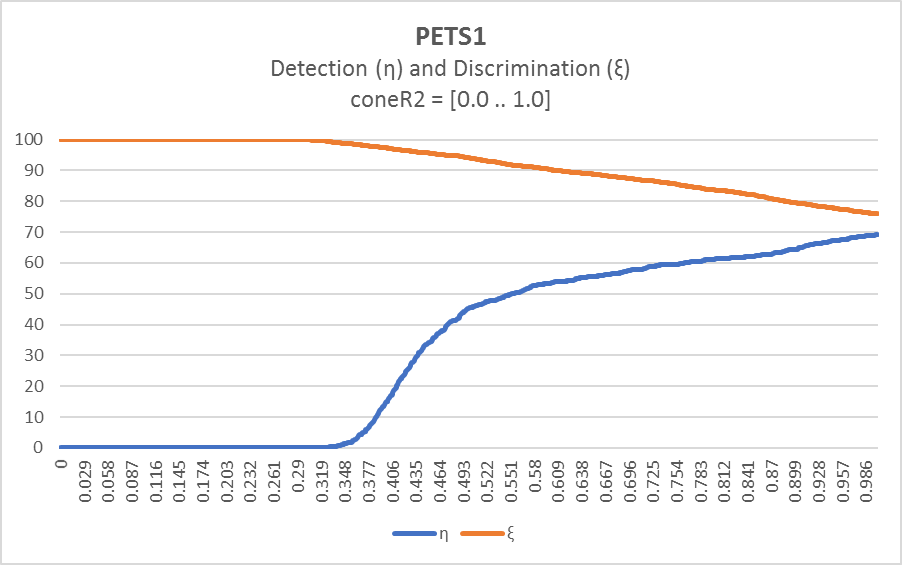
\includegraphics[width=1\linewidth]{figures/appendix/pets1_coneR2_response.jpg}
  \caption{PETS1}
\end{subfigure}
\hfill
\begin{subfigure}{.45\linewidth}
  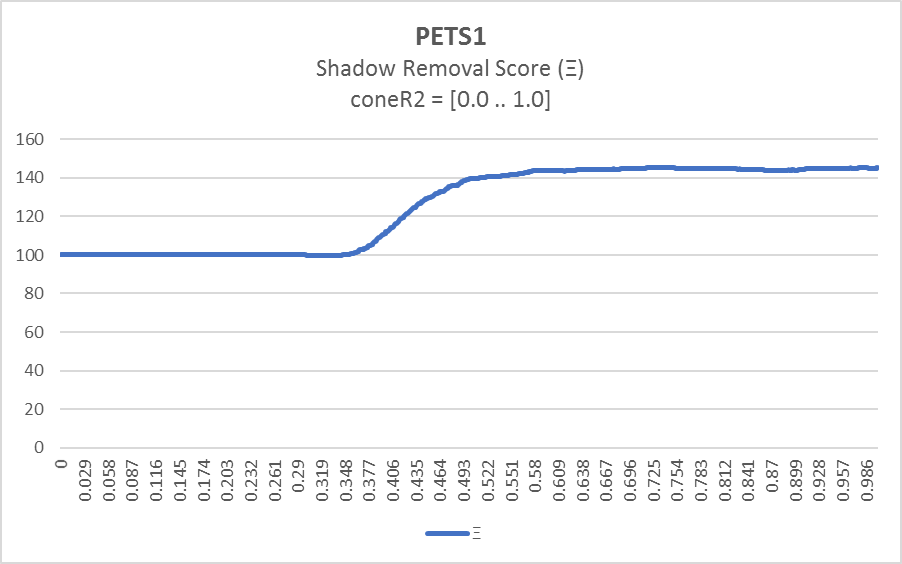
\includegraphics[width=1\linewidth]{figures/appendix/pets1_coneR2_score.jpg}
  \caption{PETS1}
\end{subfigure}
\hfill
\begin{subfigure}{.45\linewidth}
  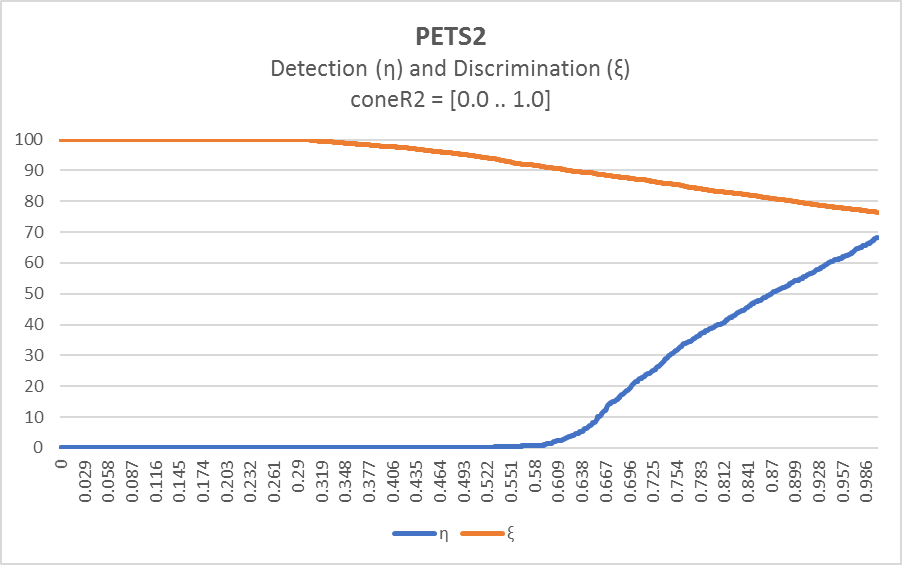
\includegraphics[width=1\linewidth]{figures/appendix/pets2_coneR2_response.jpg}
  \caption{PETS2}
\end{subfigure}
\hfill
\begin{subfigure}{.45\linewidth}
  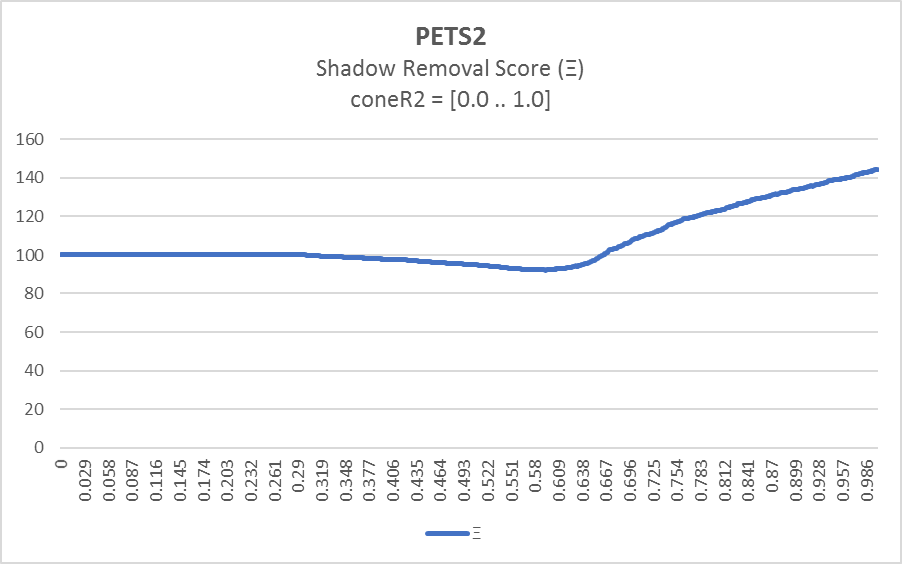
\includegraphics[width=1\linewidth]{figures/appendix/pets2_coneR2_score.jpg}
  \caption{PETS2}
\end{subfigure}
\caption{Detection (blue) and discrimination (orange) rates are calculated as the value of \textit{coneR2} is varied from [0.0 .. 1.0]. (pt. 1 of 4)}

\end{sidewaysfigure}

% hw1/hw3
\begin{sidewaysfigure}

  \begin{subfigure}{.45\linewidth}
  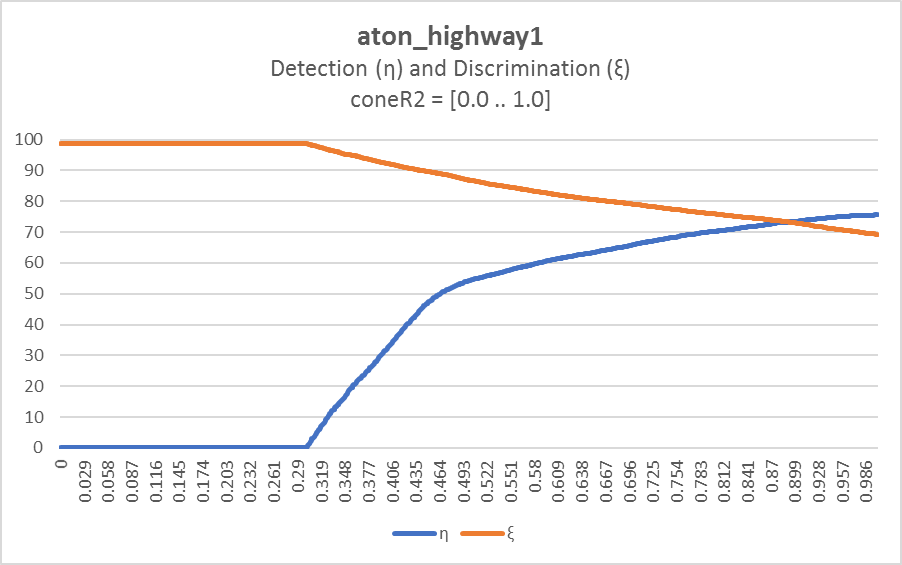
\includegraphics[width=1\linewidth]{figures/appendix/highway1_coneR2_response.jpg}
  \caption{aton\_highway1}
\end{subfigure}
\hfill
\begin{subfigure}{.45\linewidth}
  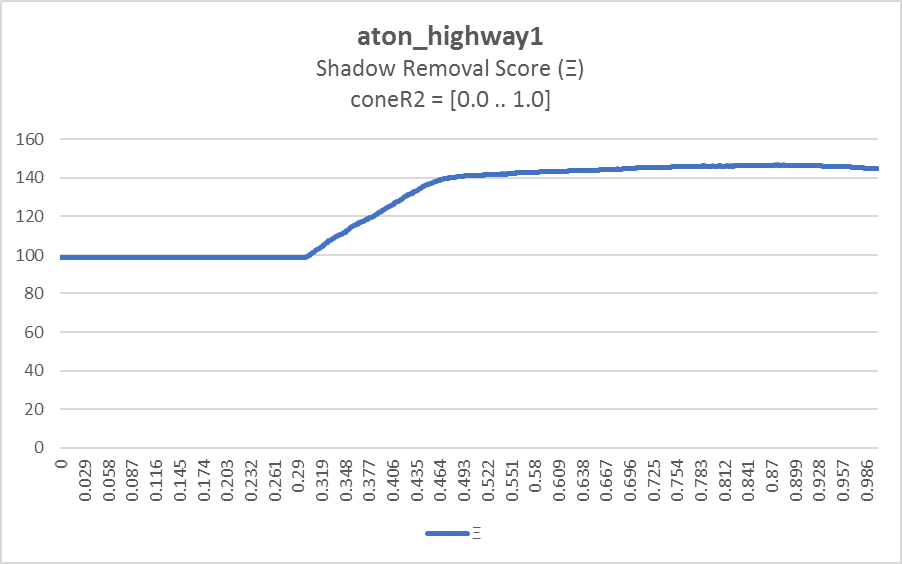
\includegraphics[width=1\linewidth]{figures/appendix/highway1_coneR2_score.jpg}
  \caption{aton\_highway1}
\end{subfigure}
\hfill
\begin{subfigure}{.45\linewidth}
  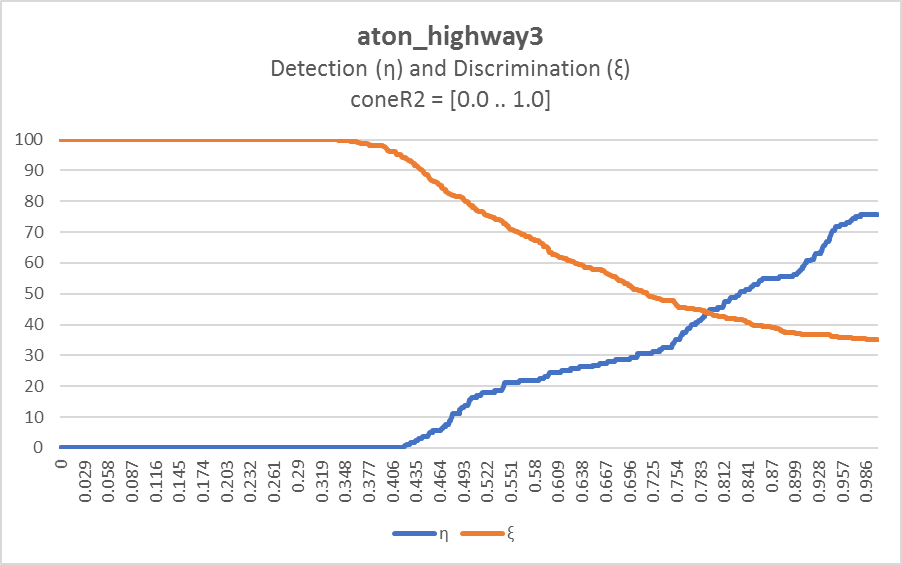
\includegraphics[width=1\linewidth]{figures/appendix/highway3_coneR2_response.jpg}
  \caption{aton\_highway3}
\end{subfigure}
\hfill
\begin{subfigure}{.45\linewidth}
  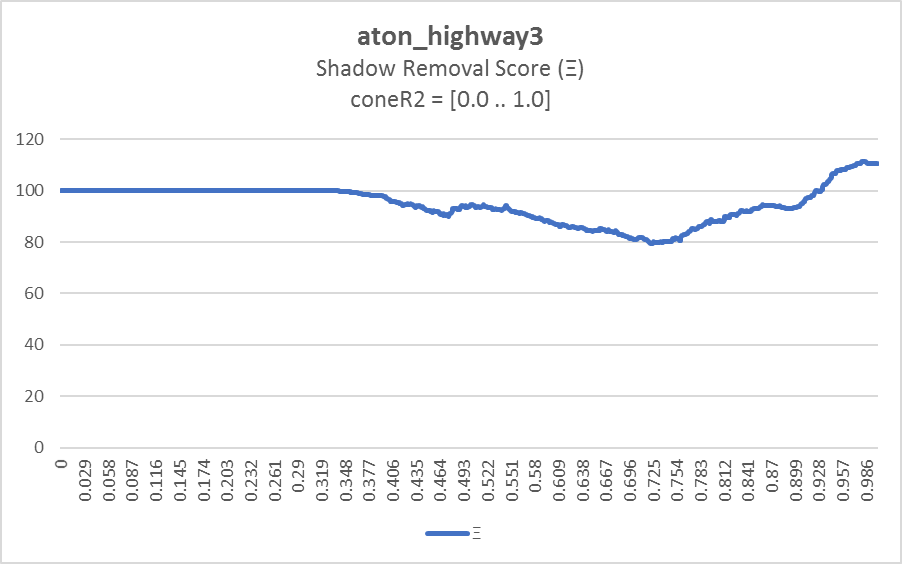
\includegraphics[width=1\linewidth]{figures/appendix/highway3_coneR2_score.jpg}
  \caption{aton\_highway3}
\end{subfigure}
\caption{Detection (blue) and discrimination (orange) rates are calculated as the value of \textit{coneR2} is varied from [0.0 .. 1.0]. (pt. 2 of 4)}

\end{sidewaysfigure}

% room/campus
\begin{sidewaysfigure}

  \begin{subfigure}{.45\linewidth}
  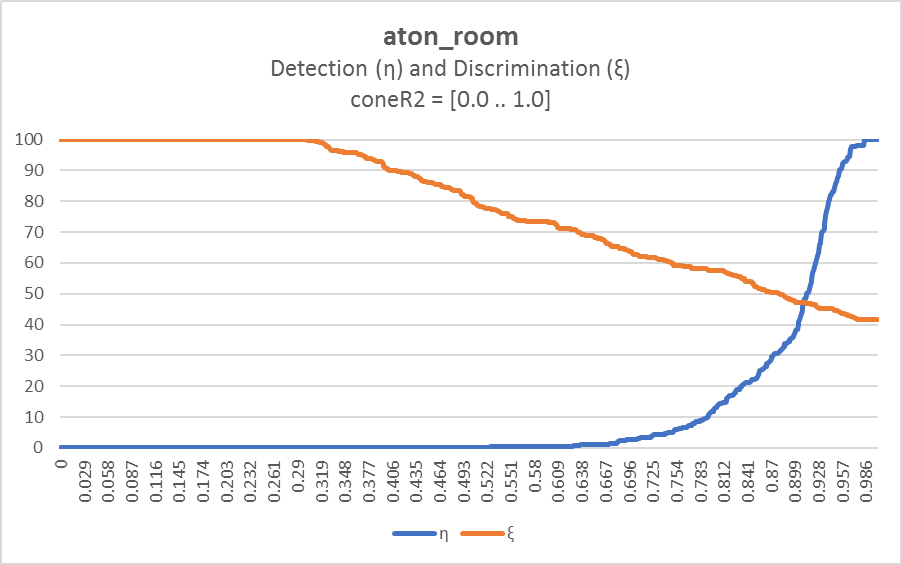
\includegraphics[width=1\linewidth]{figures/appendix/room_coneR2_response.jpg}
  \caption{aton\_room}
\end{subfigure}
\hfill
\begin{subfigure}{.45\linewidth}
  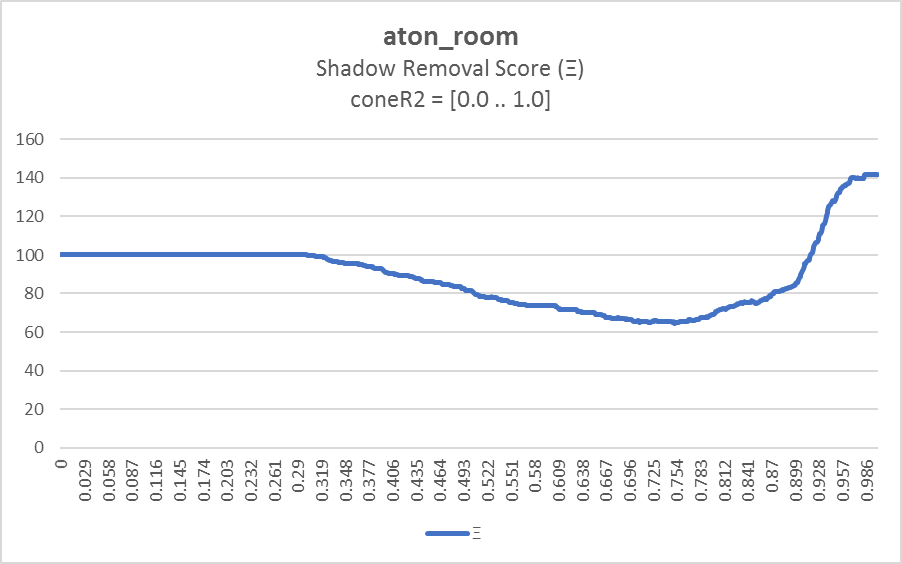
\includegraphics[width=1\linewidth]{figures/appendix/room_coneR2_score.jpg}
  \caption{aton\_room}
\end{subfigure}
\hfill
\begin{subfigure}{.45\linewidth}
  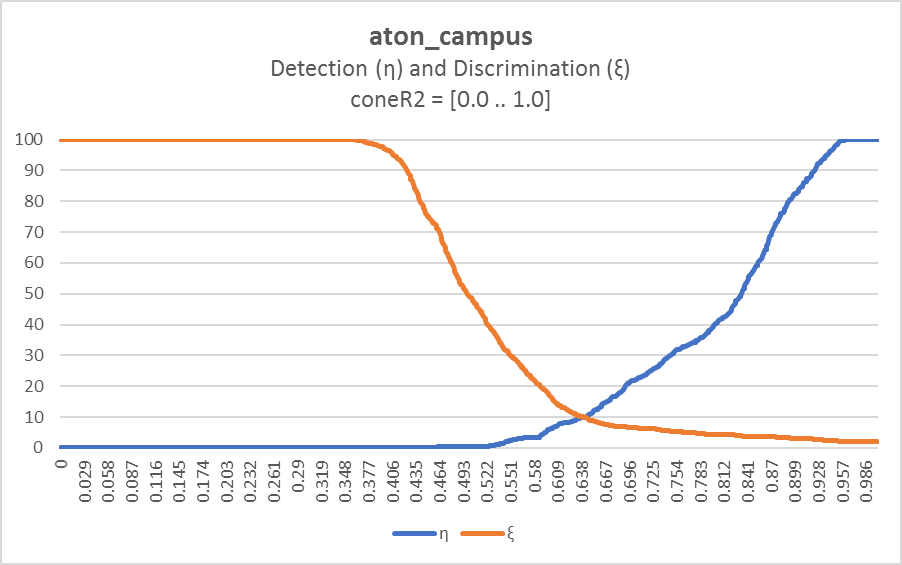
\includegraphics[width=1\linewidth]{figures/appendix/campus_coneR2_response.jpg}
  \caption{aton\_campus}
\end{subfigure}
\hfill
\begin{subfigure}{.45\linewidth}
  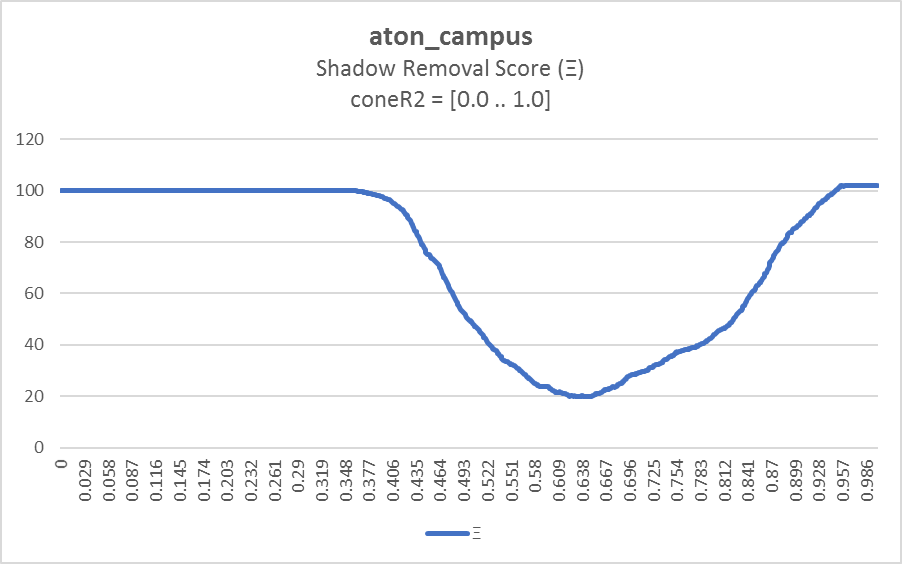
\includegraphics[width=1\linewidth]{figures/appendix/campus_coneR2_score.jpg}
  \caption{aton\_campus}
\end{subfigure}
\caption{Detection (blue) and discrimination (orange) rates are calculated as the value of \textit{coneR2} is varied from [0.0 .. 1.0]. (pt. 3 of 4)}

\end{sidewaysfigure}

% hallway/lab
\begin{sidewaysfigure}

  \begin{subfigure}{.45\linewidth}
  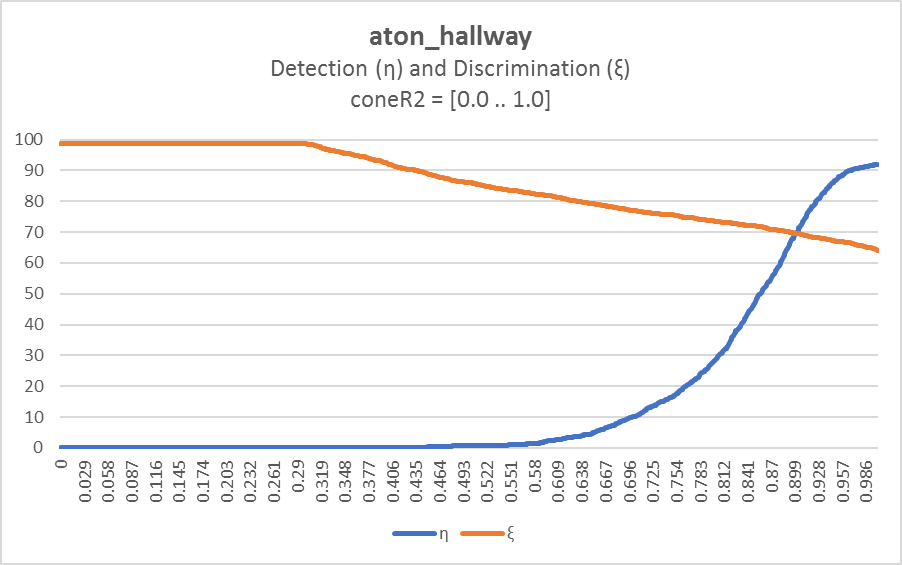
\includegraphics[width=1\linewidth]{figures/appendix/hallway_coneR2_response.jpg}
  \caption{aton\_hallway}
\end{subfigure}
\hfill
\begin{subfigure}{.45\linewidth}
  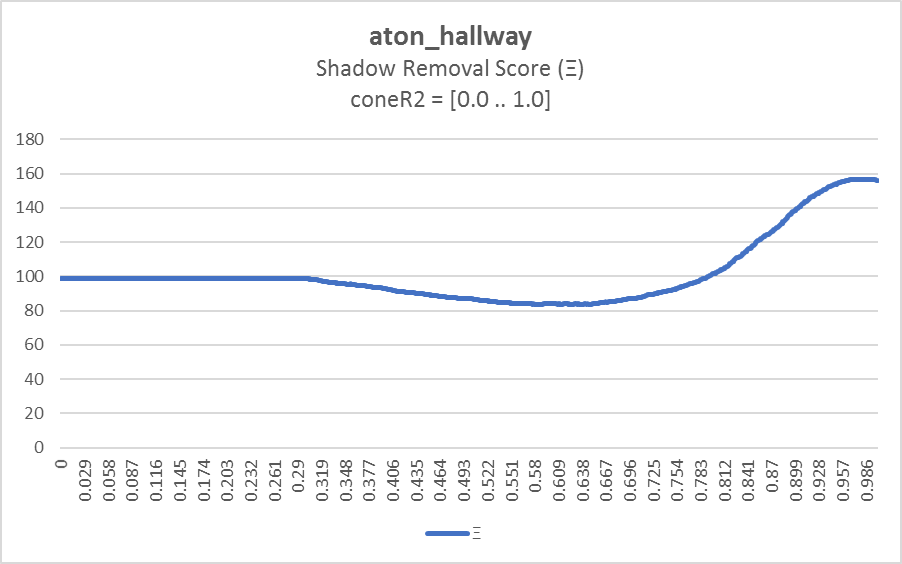
\includegraphics[width=1\linewidth]{figures/appendix/hallway_coneR2_score.jpg}
  \caption{aton\_hallway}
\end{subfigure}
\hfill
\begin{subfigure}{.45\linewidth}
  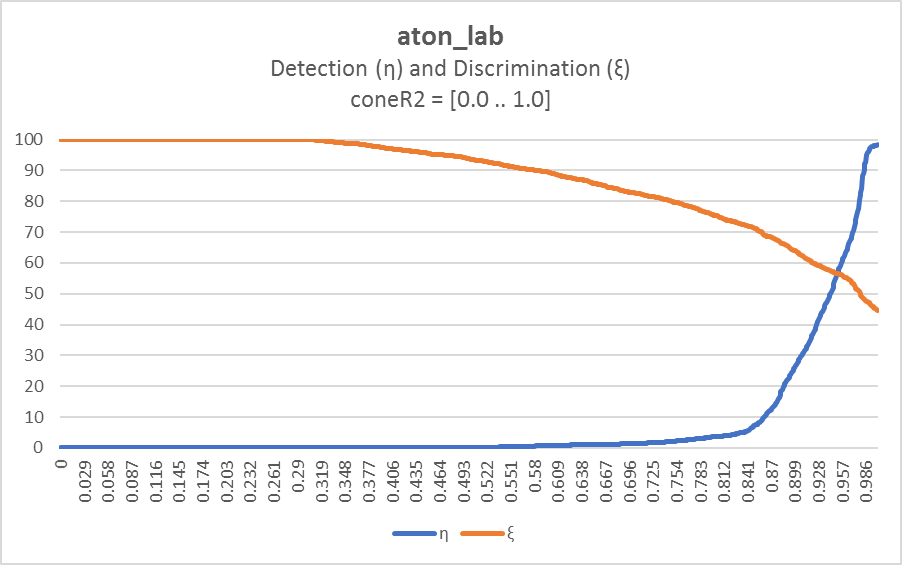
\includegraphics[width=1\linewidth]{figures/appendix/lab_coneR2_response.jpg}
  \caption{aton\_lab}
\end{subfigure}
\hfill
\begin{subfigure}{.45\linewidth}
  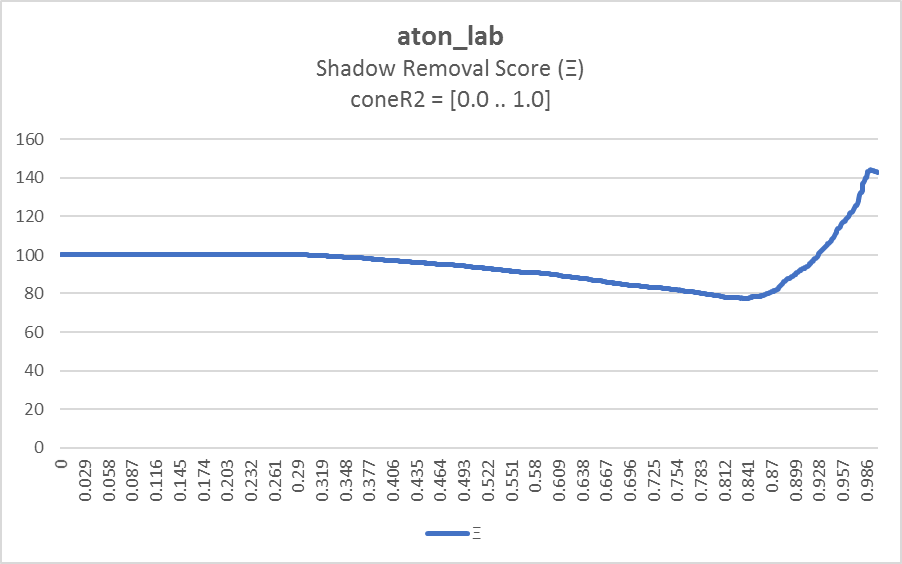
\includegraphics[width=1\linewidth]{figures/appendix/lab_coneR2_score.jpg}
  \caption{aton\_lab}
\end{subfigure}
\caption{Detection (blue) and discrimination (orange) rates are calculated as the value of \textit{coneR2} is varied from [0.0 .. 1.0]. (pt. 4 of 4)}

\end{sidewaysfigure}

\clearpage
\FloatBarrier
% coneAngle [0.0 .. 1.0] dd
% coneAngle [0.0 .. 1.0] score
\begin{sidewaysfigure}

  \begin{subfigure}{.45\linewidth}
  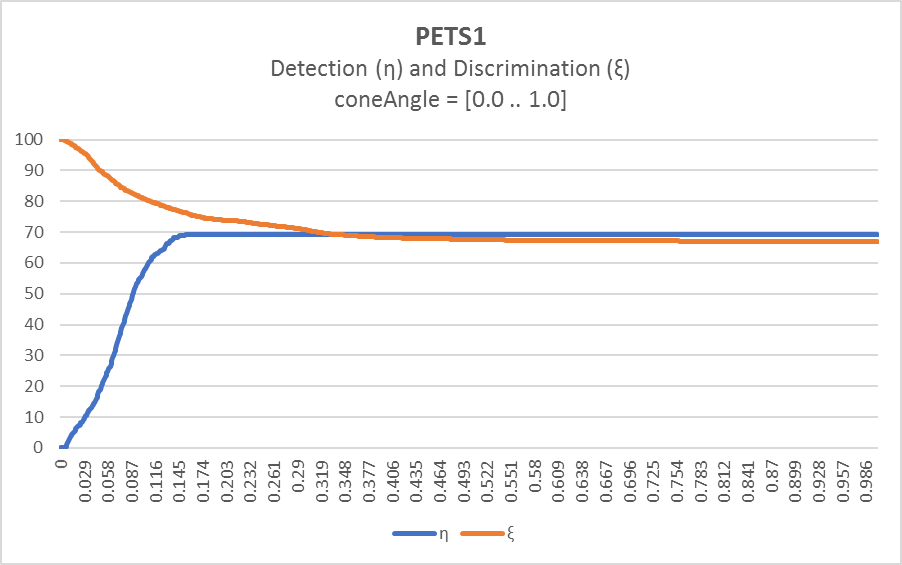
\includegraphics[width=1\linewidth]{figures/appendix/pets1_coneAngle_response.jpg}
  \caption{PETS1}
\end{subfigure}
\hfill
\begin{subfigure}{.45\linewidth}
  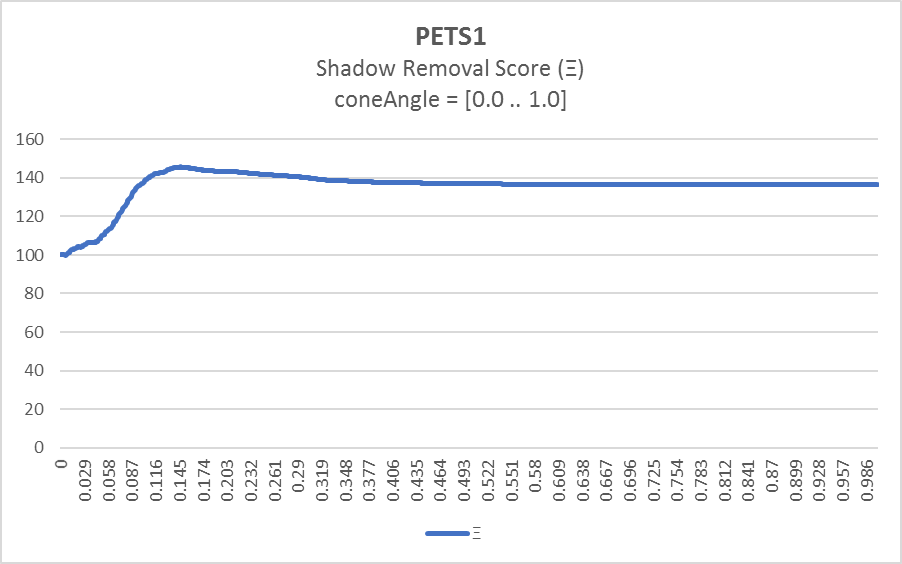
\includegraphics[width=1\linewidth]{figures/appendix/pets1_coneAngle_score.jpg}
  \caption{PETS1}
\end{subfigure}
\hfill
\begin{subfigure}{.45\linewidth}
  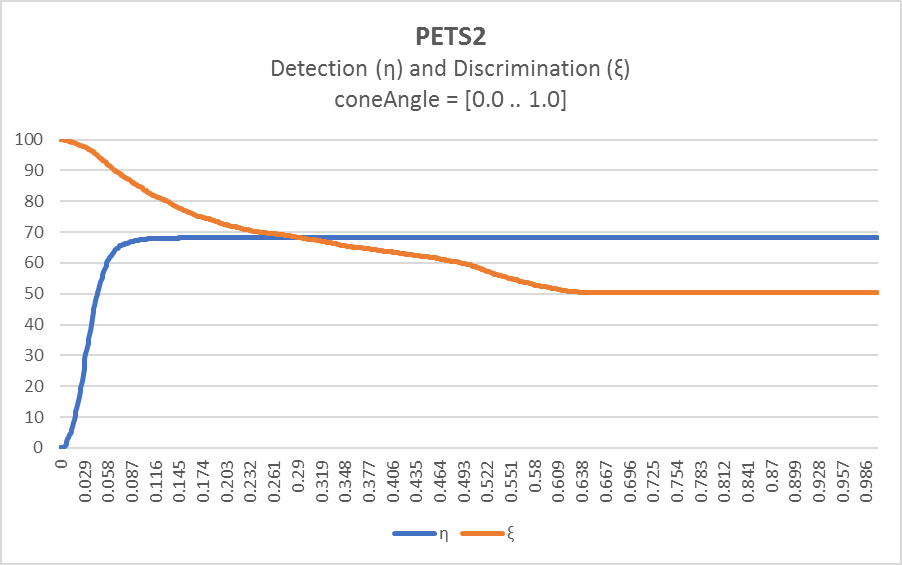
\includegraphics[width=1\linewidth]{figures/appendix/pets2_coneAngle_response.jpg}
  \caption{PETS2}
\end{subfigure}
\hfill
\begin{subfigure}{.45\linewidth}
  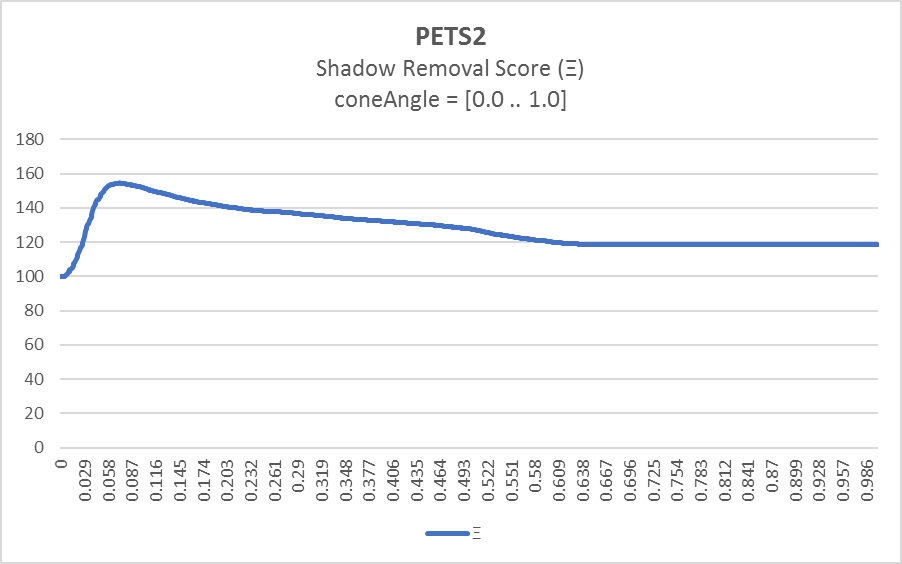
\includegraphics[width=1\linewidth]{figures/appendix/pets2_coneAngle_score.jpg}
  \caption{PETS2}
\end{subfigure}
\caption{Detection (blue) and discrimination (orange) rates are calculated as the value of \textit{coneAngle} is varied from [0.0 .. 1.0]. (pt. 1 of 4)}

\end{sidewaysfigure}

% hw1/hw3
\begin{sidewaysfigure}

  \begin{subfigure}{.45\linewidth}
  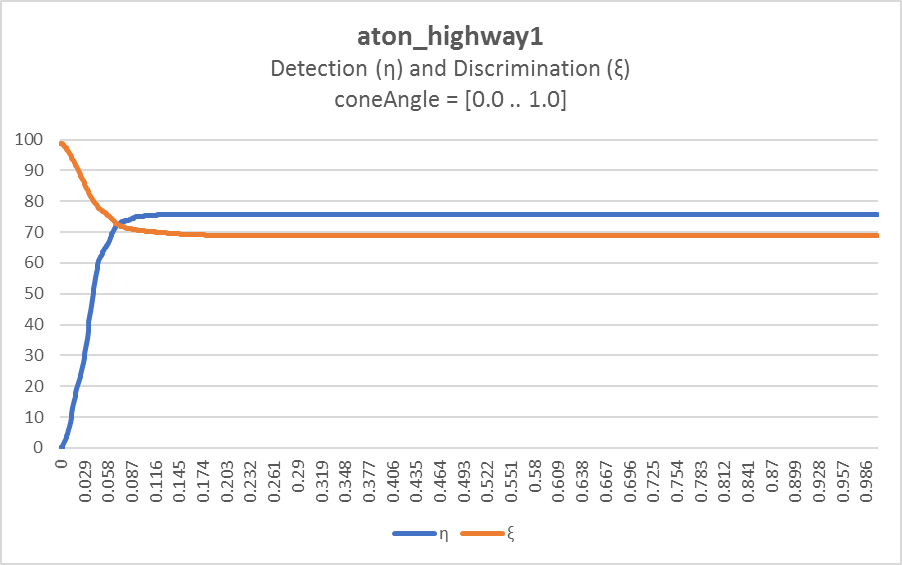
\includegraphics[width=1\linewidth]{figures/appendix/highway1_coneAngle_response.jpg}
  \caption{aton\_highway1}
\end{subfigure}
\hfill
\begin{subfigure}{.45\linewidth}
  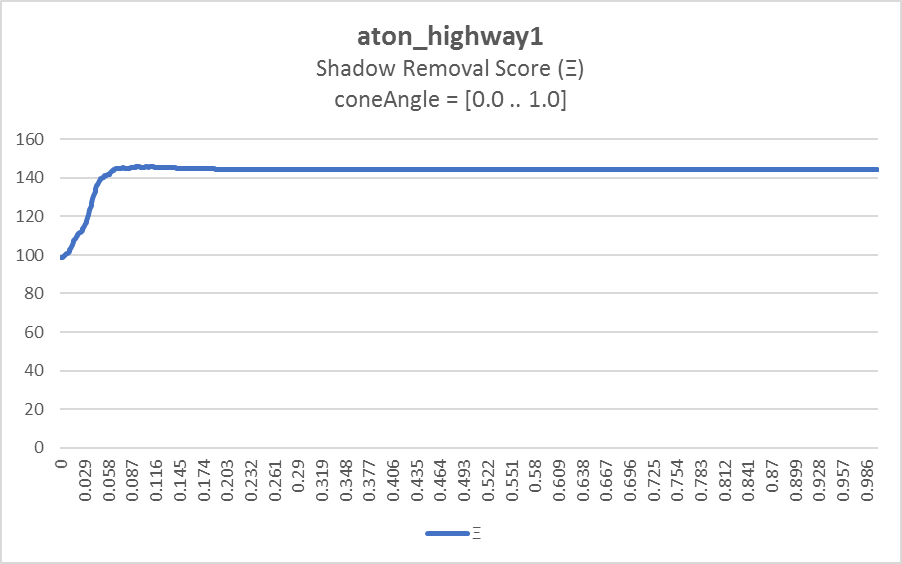
\includegraphics[width=1\linewidth]{figures/appendix/highway1_coneAngle_score.jpg}
  \caption{aton\_highway1}
\end{subfigure}
\hfill
\begin{subfigure}{.45\linewidth}
  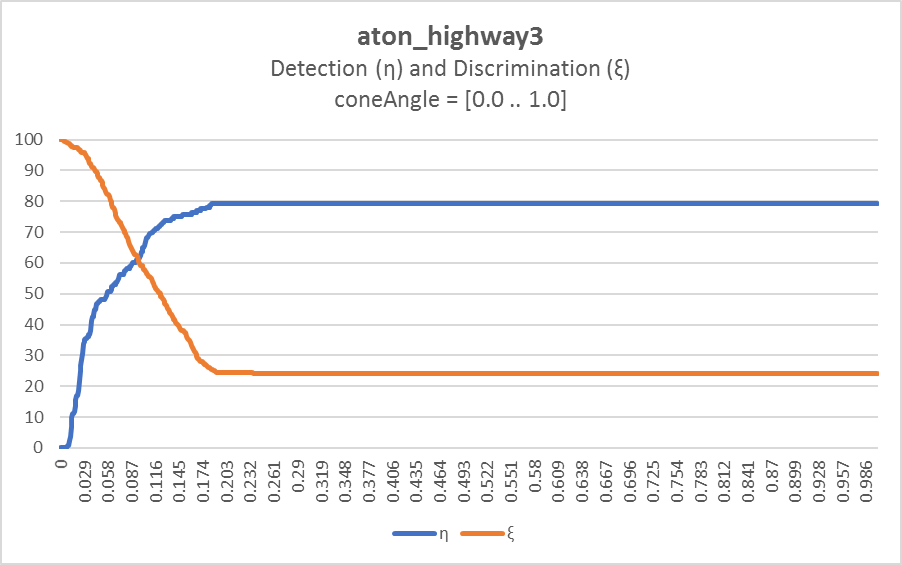
\includegraphics[width=1\linewidth]{figures/appendix/highway3_coneAngle_response.jpg}
  \caption{aton\_highway3}
\end{subfigure}
\hfill
\begin{subfigure}{.45\linewidth}
  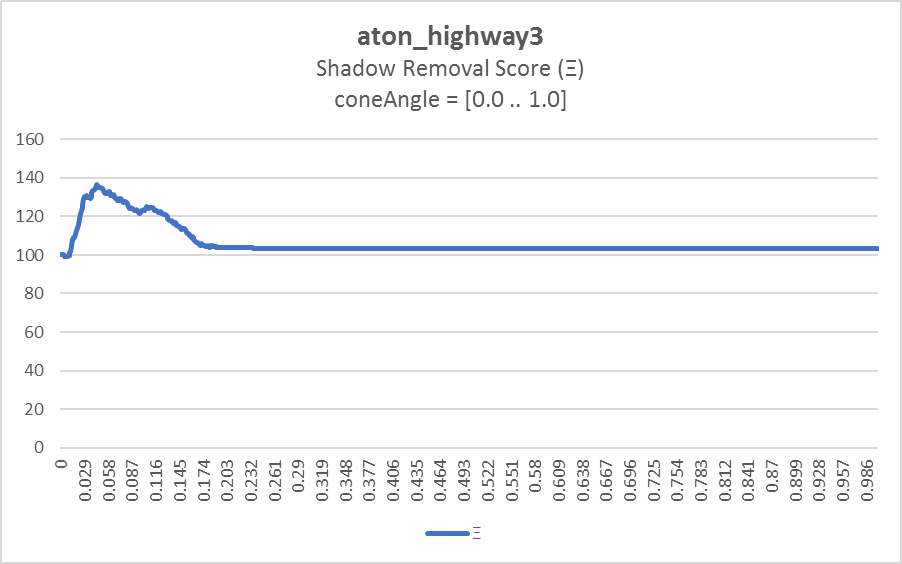
\includegraphics[width=1\linewidth]{figures/appendix/highway3_coneAngle_score.jpg}
  \caption{aton\_highway3}
\end{subfigure}
\caption{Detection (blue) and discrimination (orange) rates are calculated as the value of \textit{coneAngle} is varied from [0.0 .. 1.0]. (pt. 2 of 4)}

\end{sidewaysfigure}

% room/campus
\begin{sidewaysfigure}

  \begin{subfigure}{.45\linewidth}
  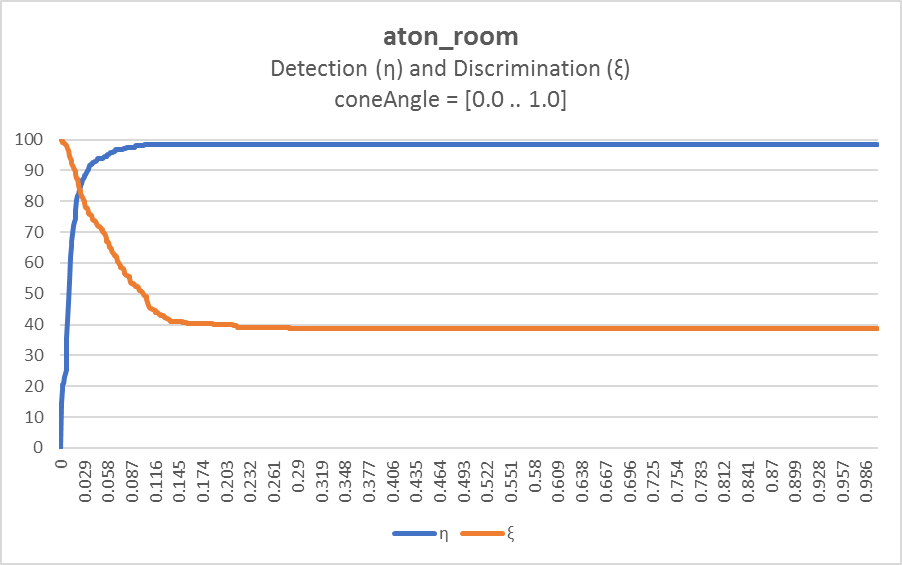
\includegraphics[width=1\linewidth]{figures/appendix/room_coneAngle_response.jpg}
  \caption{aton\_room}
\end{subfigure}
\hfill
\begin{subfigure}{.45\linewidth}
  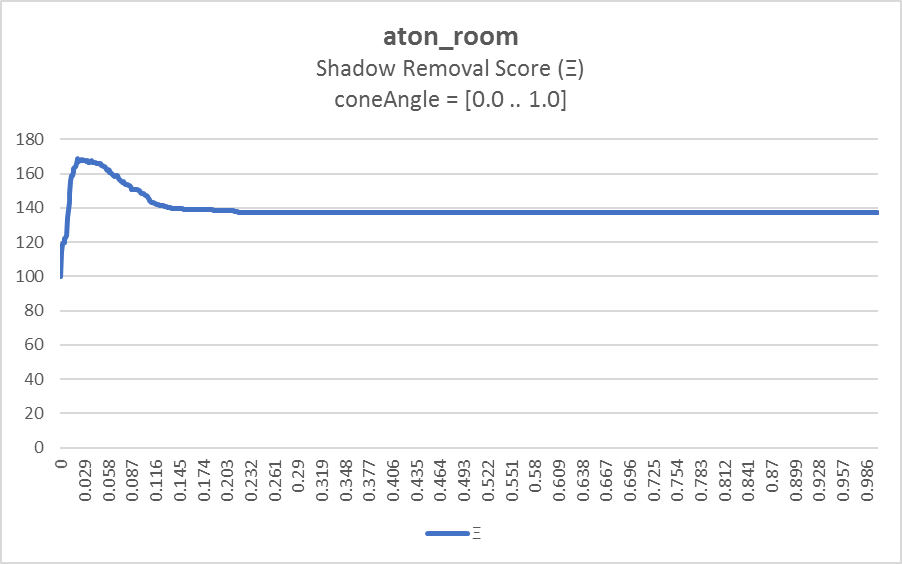
\includegraphics[width=1\linewidth]{figures/appendix/room_coneAngle_score.jpg}
  \caption{aton\_room}
\end{subfigure}
\hfill
\begin{subfigure}{.45\linewidth}
  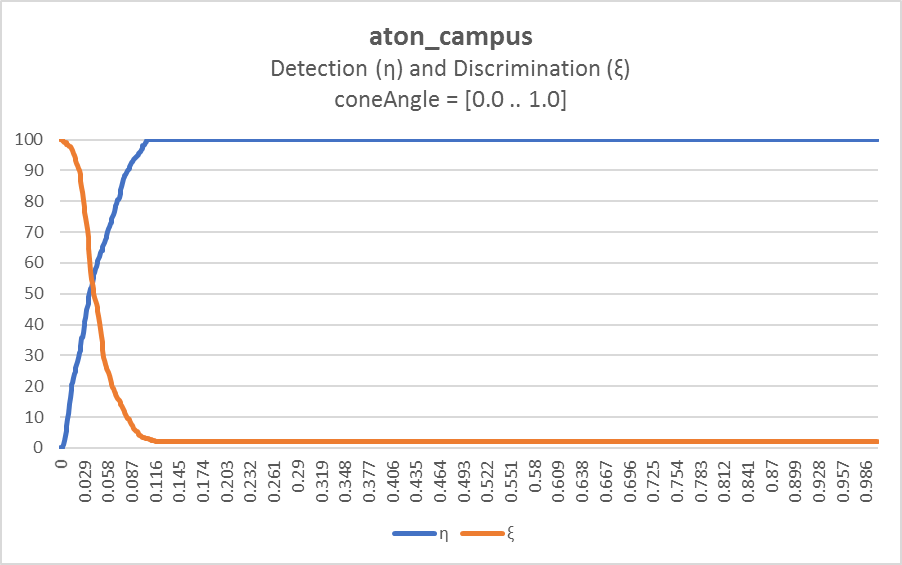
\includegraphics[width=1\linewidth]{figures/appendix/campus_coneAngle_response.jpg}
  \caption{aton\_campus}
\end{subfigure}
\hfill
\begin{subfigure}{.45\linewidth}
  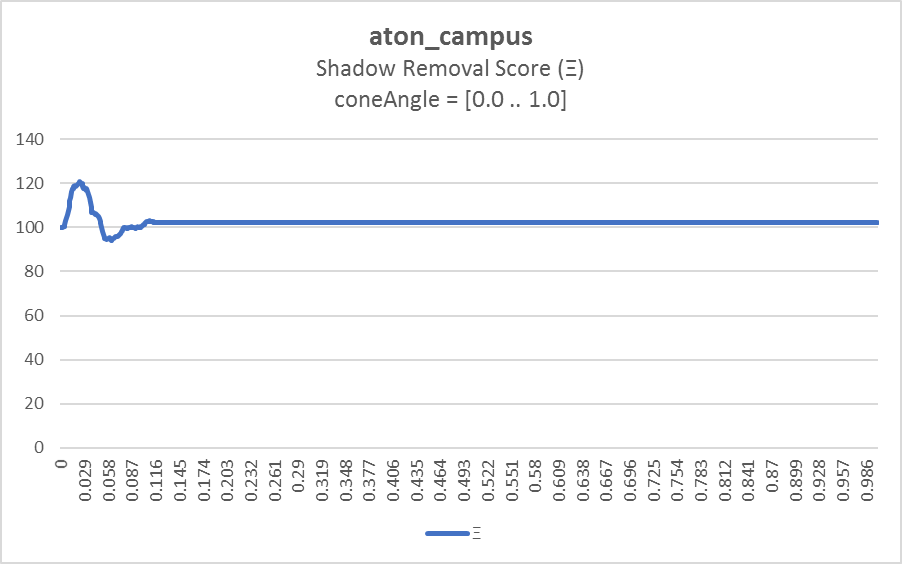
\includegraphics[width=1\linewidth]{figures/appendix/campus_coneAngle_score.jpg}
  \caption{aton\_campus}
\end{subfigure}
\caption{Detection (blue) and discrimination (orange) rates are calculated as the value of \textit{coneAngle} is varied from [0.0 .. 1.0]. (pt. 3 of 4)}

\end{sidewaysfigure}

% hallway/lab
\begin{sidewaysfigure}

  \begin{subfigure}{.45\linewidth}
  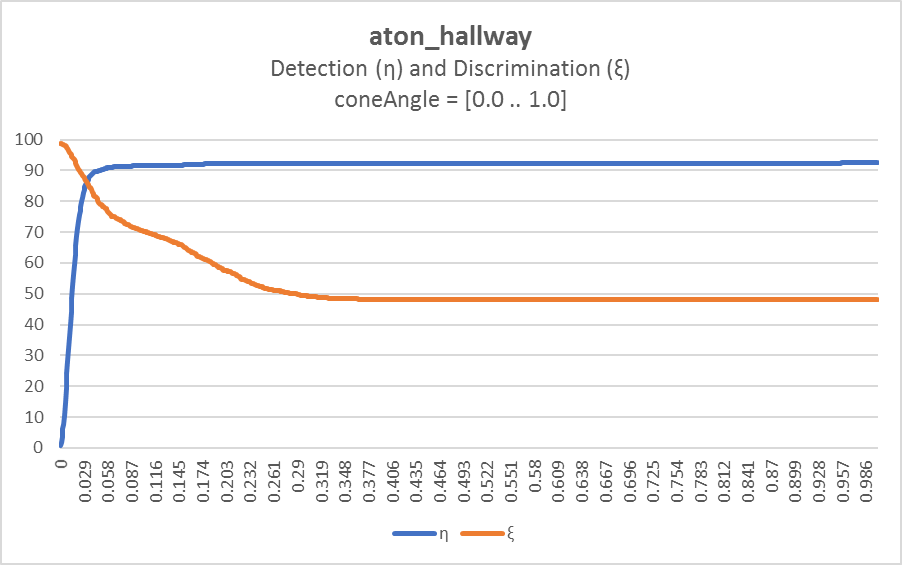
\includegraphics[width=1\linewidth]{figures/appendix/hallway_coneAngle_response.jpg}
  \caption{aton\_hallway}
\end{subfigure}
\hfill
\begin{subfigure}{.45\linewidth}
  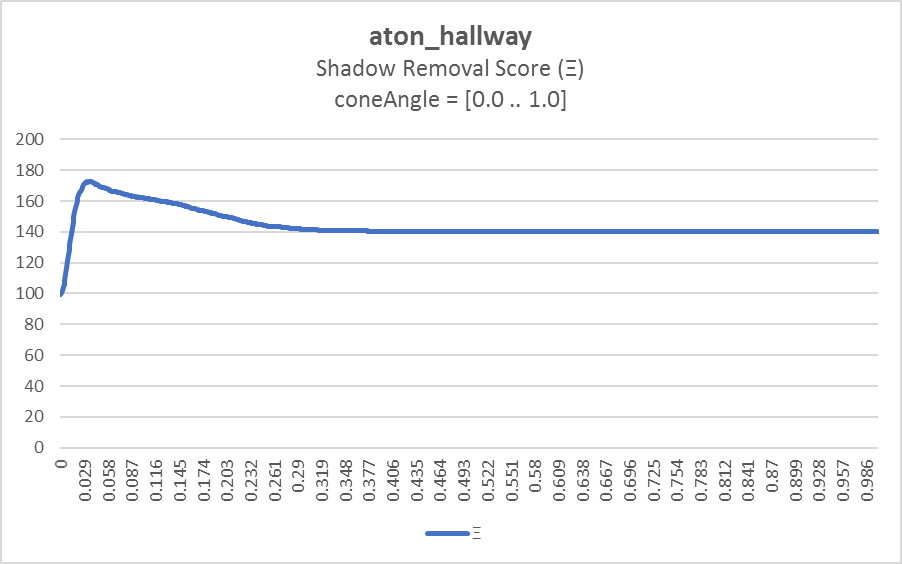
\includegraphics[width=1\linewidth]{figures/appendix/hallway_coneAngle_score.jpg}
  \caption{aton\_hallway}
\end{subfigure}
\hfill
\begin{subfigure}{.45\linewidth}
  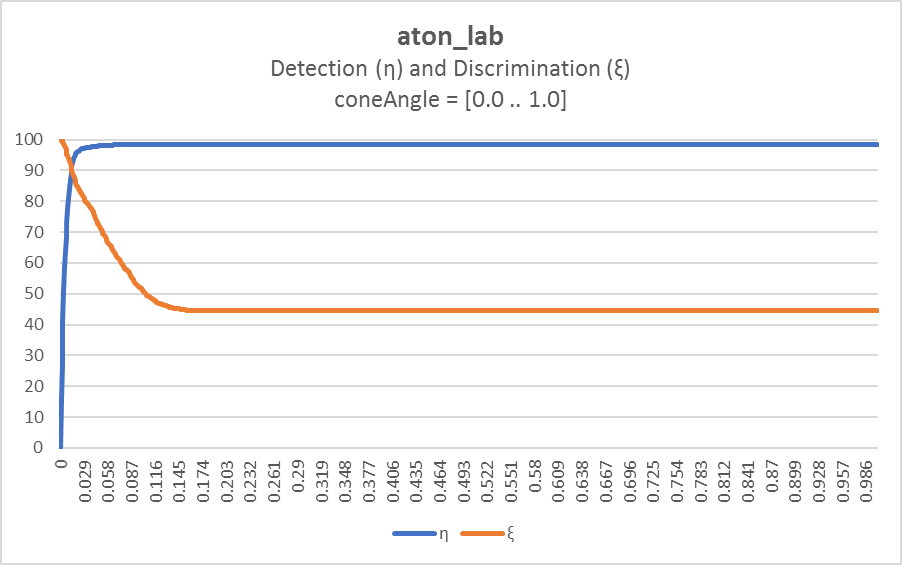
\includegraphics[width=1\linewidth]{figures/appendix/lab_coneAngle_response.jpg}
  \caption{aton\_lab}
\end{subfigure}
\hfill
\begin{subfigure}{.45\linewidth}
  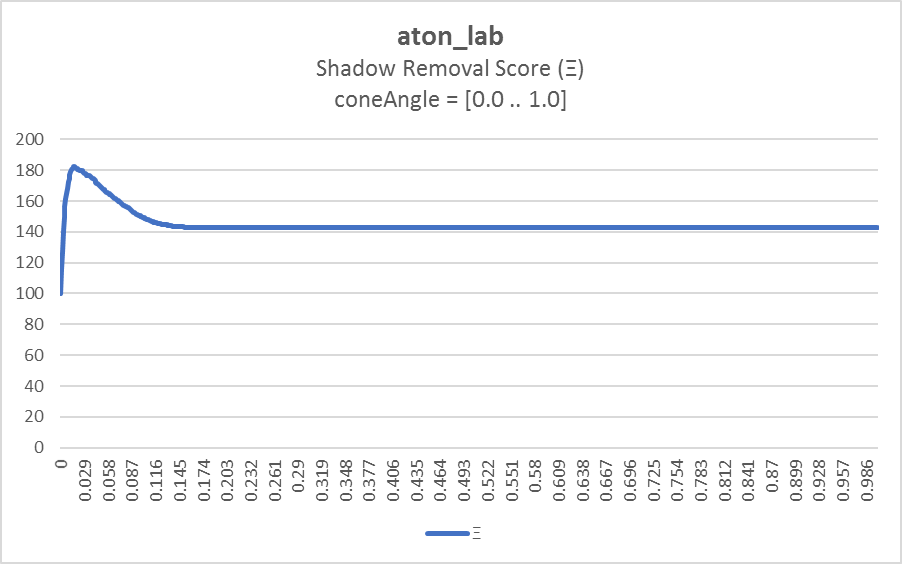
\includegraphics[width=1\linewidth]{figures/appendix/lab_coneAngle_score.jpg}
  \caption{aton\_lab}
\end{subfigure}
\caption{Detection (blue) and discrimination (orange) rates are calculated as the value of \textit{coneAngle} is varied from [0.0 .. 1.0]. (pt. 4 of 4)}

\end{sidewaysfigure}

\clearpage
\FloatBarrier
% atten db
% 1-4
\begin{sidewaysfigure}

  \begin{subfigure}{.45\linewidth}
  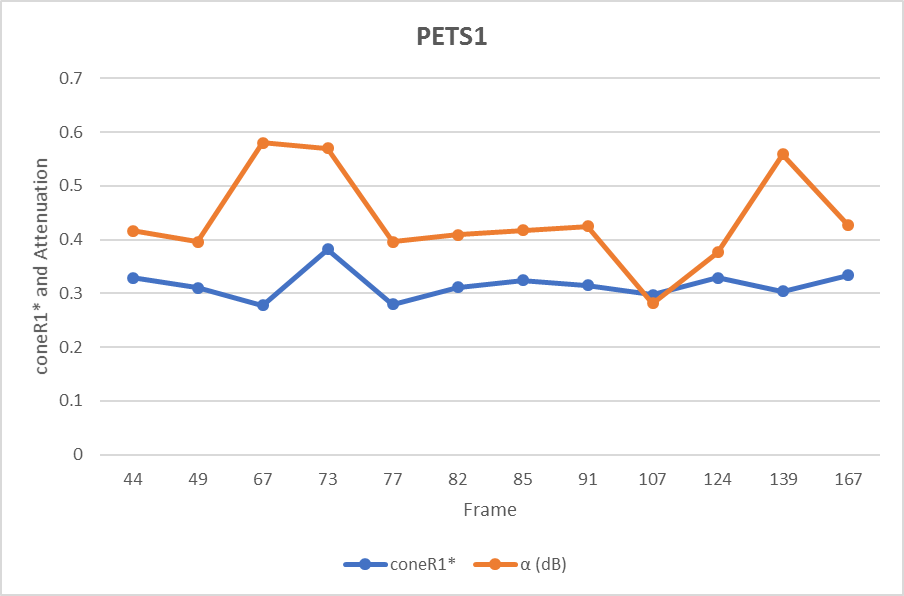
\includegraphics[width=1\linewidth]{figures/appendix/pets1_db.jpg}
  \caption{PETS1}
\end{subfigure}
\hfill
\begin{subfigure}{.45\linewidth}
  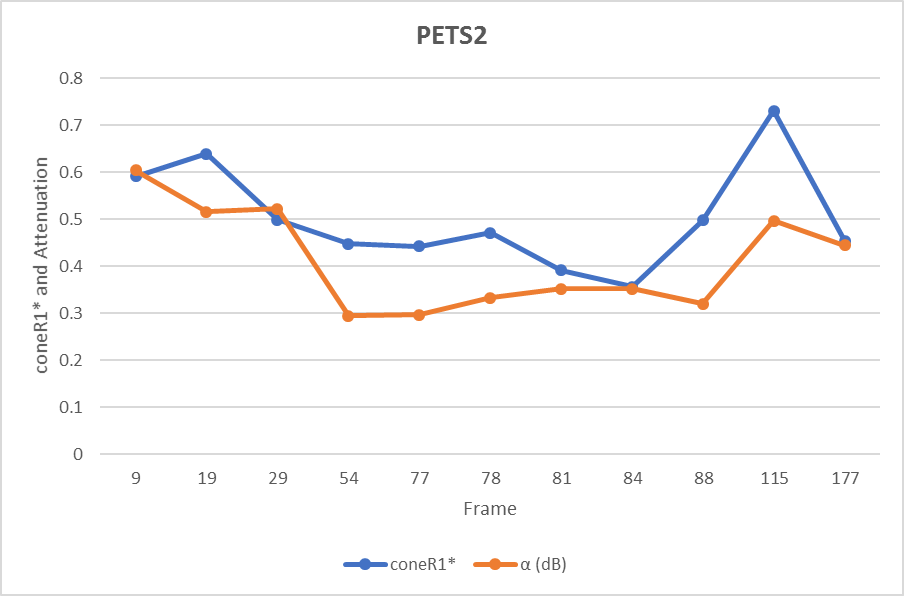
\includegraphics[width=1\linewidth]{figures/appendix/pets2_db.jpg}
  \caption{PETS2}
\end{subfigure}
\hfill
\begin{subfigure}{.45\linewidth}
  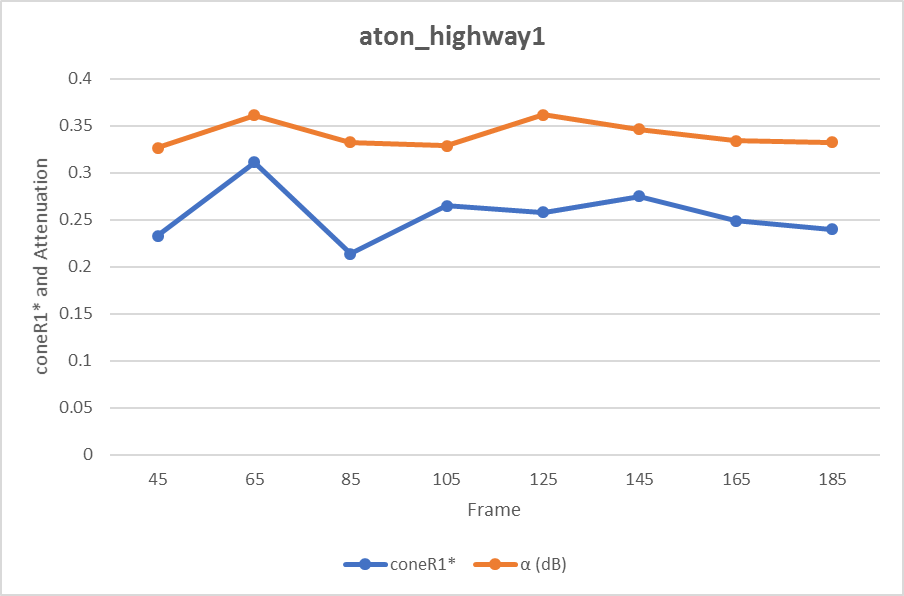
\includegraphics[width=1\linewidth]{figures/appendix/highway1_db.jpg}
  \caption{aton\_highway1}
\end{subfigure}
\hfill
\begin{subfigure}{.45\linewidth}
  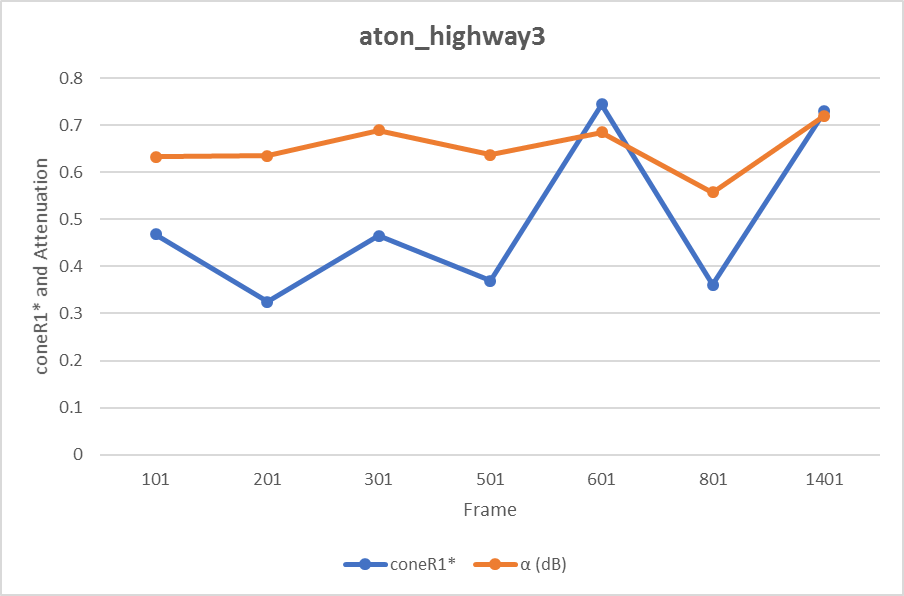
\includegraphics[width=1\linewidth]{figures/appendix/highway3_db.jpg}
  \caption{aton\_highway3}
\end{subfigure}
\caption{Attenuation ($\alpha_{dB}$ model) plotted against \textit{coneR1}*. (pt. 1 of 2)}

\end{sidewaysfigure}

% 5-8
\begin{sidewaysfigure}

  \begin{subfigure}{.45\linewidth}
  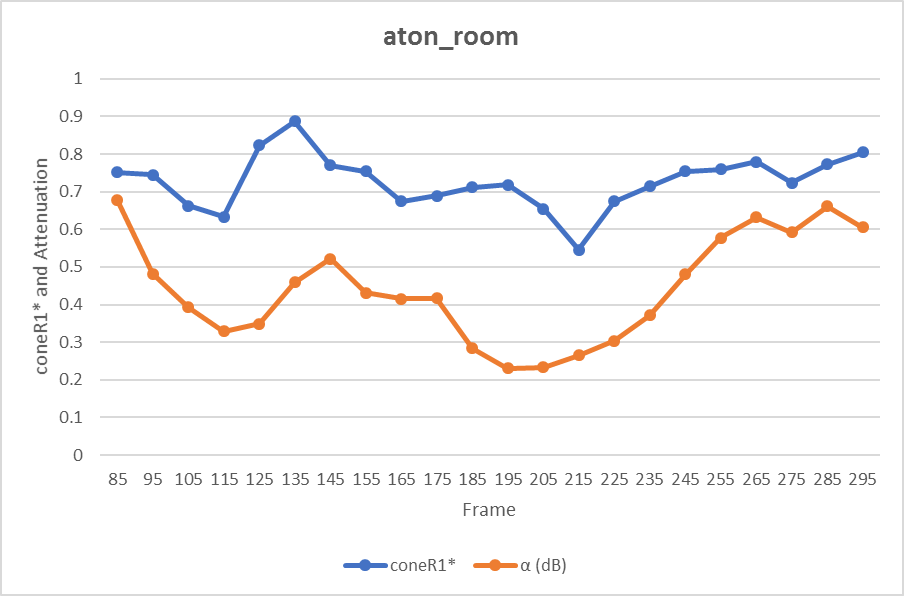
\includegraphics[width=1\linewidth]{figures/appendix/room_db.jpg}
  \caption{aton\_room}
\end{subfigure}
\hfill
\begin{subfigure}{.45\linewidth}
  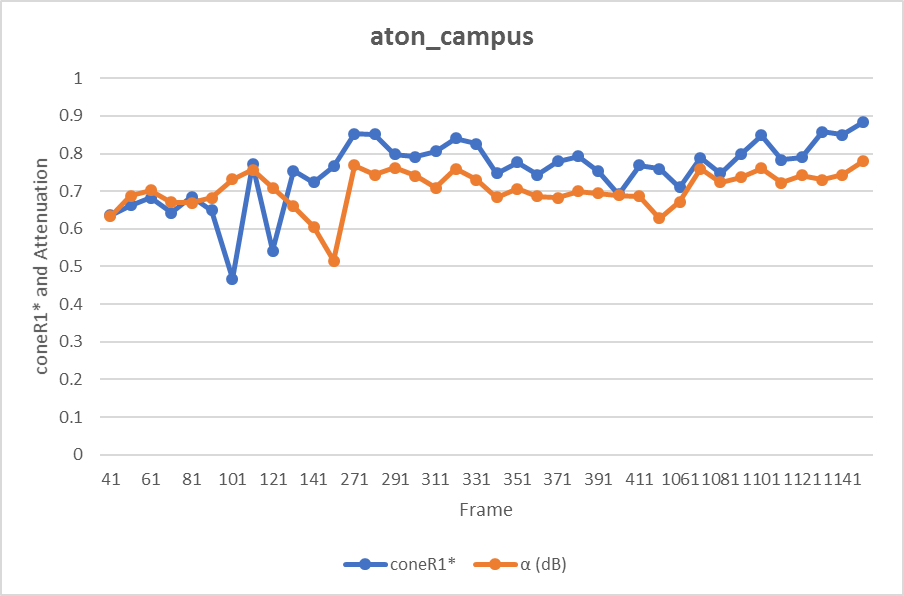
\includegraphics[width=1\linewidth]{figures/appendix/campus_db.jpg}
  \caption{aton\_campus}
\end{subfigure}
\hfill
\begin{subfigure}{.45\linewidth}
  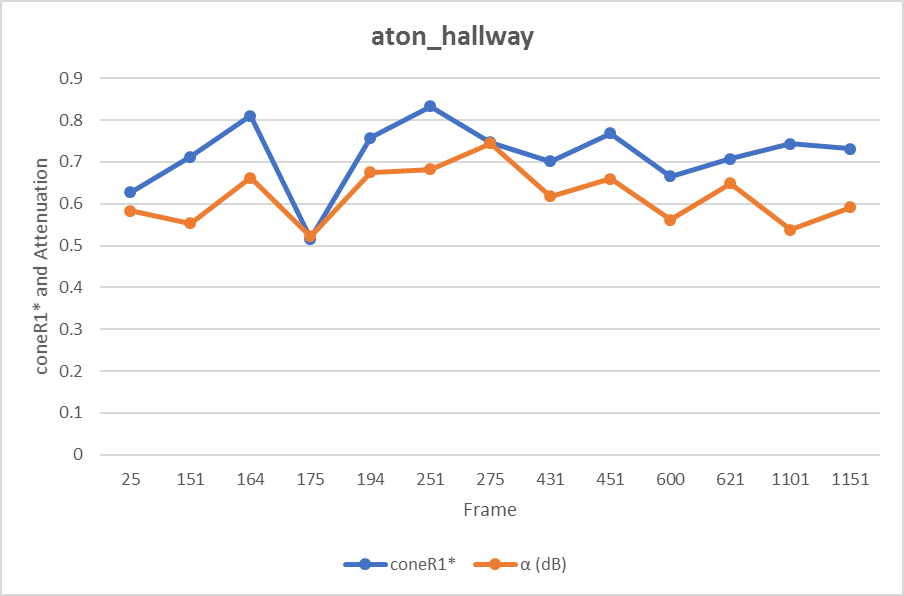
\includegraphics[width=1\linewidth]{figures/appendix/hallway_db.jpg}
  \caption{aton\_hallway}
\end{subfigure}
\hfill
\begin{subfigure}{.45\linewidth}
  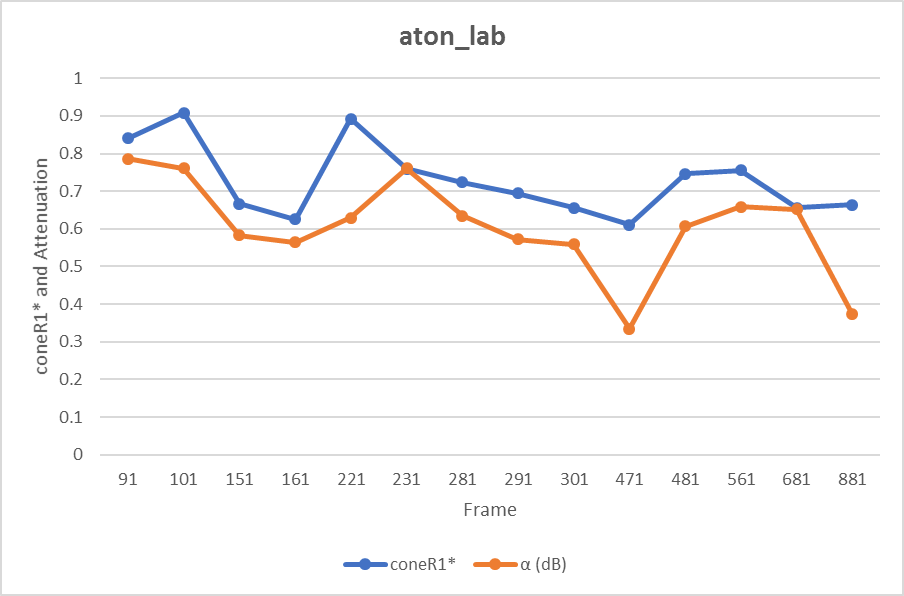
\includegraphics[width=1\linewidth]{figures/appendix/lab_db.jpg}
  \caption{aton\_lab}
\end{subfigure}
\caption{Attenuation ($\alpha_{dB}$ model) plotted against \textit{coneR1}*. (pt. 2 of 2)}

\end{sidewaysfigure}

\chapter{Results}
\clearpage
\FloatBarrier
% atten rgb
% 1-4
\begin{sidewaysfigure}

  \begin{subfigure}{.45\linewidth}
  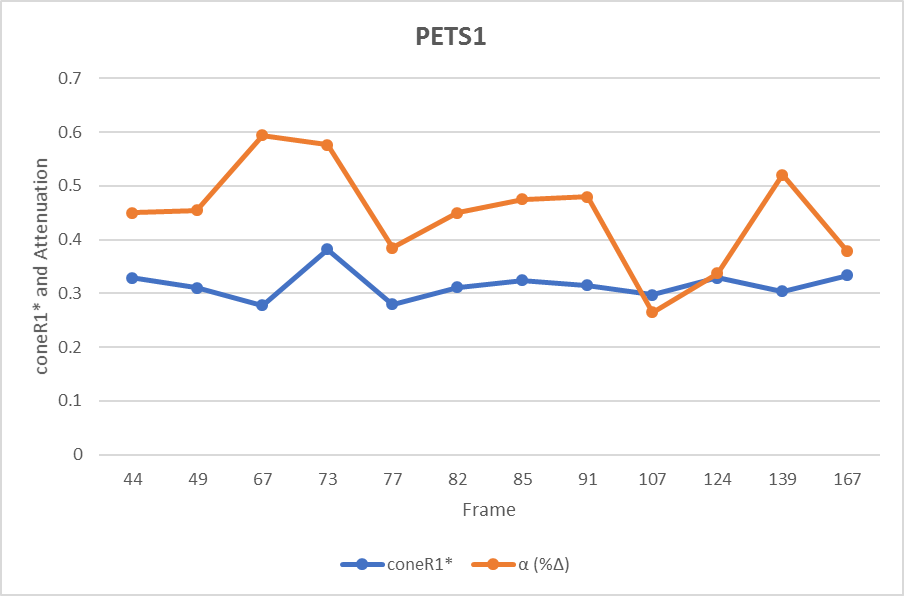
\includegraphics[width=1\linewidth]{figures/appendix/pets1_rgb.jpg}
  \caption{PETS1}
\end{subfigure}
\hfill
\begin{subfigure}{.45\linewidth}
  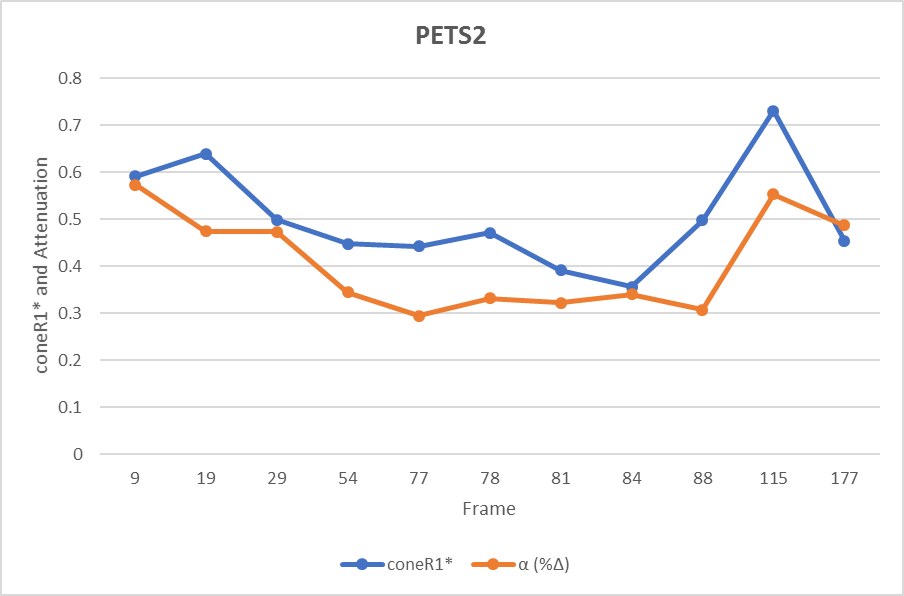
\includegraphics[width=1\linewidth]{figures/appendix/pets2_rgb.jpg}
  \caption{PETS2}
\end{subfigure}
\hfill
\begin{subfigure}{.45\linewidth}
  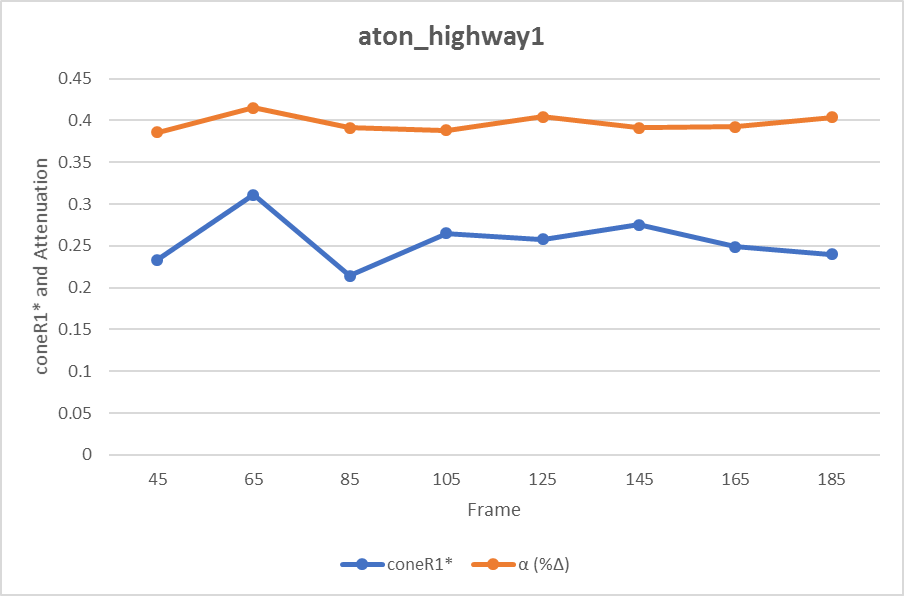
\includegraphics[width=1\linewidth]{figures/appendix/highway1_rgb.jpg}
  \caption{aton\_highway1}
\end{subfigure}
\hfill
\begin{subfigure}{.45\linewidth}
  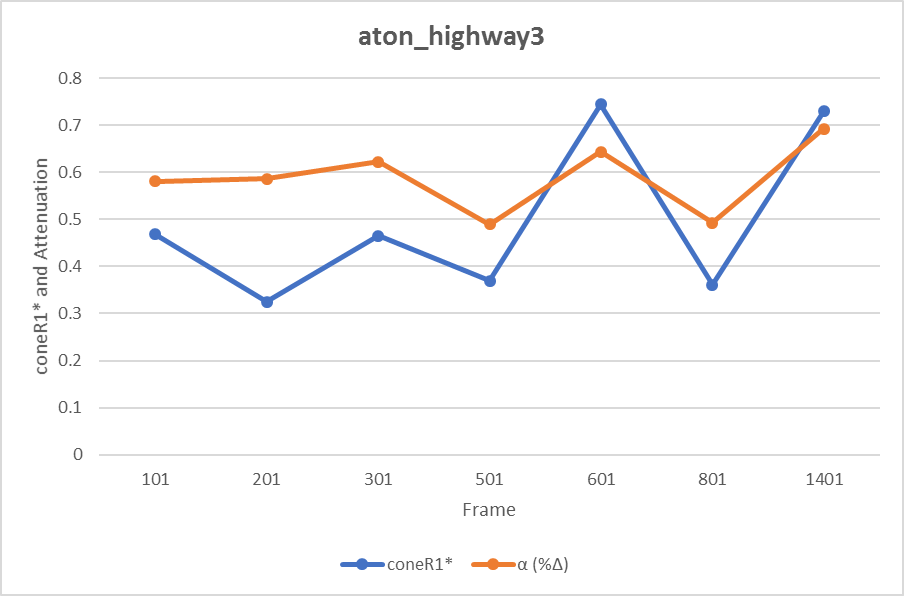
\includegraphics[width=1\linewidth]{figures/appendix/highway3_rgb.jpg}
  \caption{aton\_highway3}
\end{subfigure}
\caption{Attenuation ($\alpha_{\%\Delta}$ model) plotted against \textit{coneR1}*. (pt. 1 of 2)}

\end{sidewaysfigure}

% 5-8
\begin{sidewaysfigure}

  \begin{subfigure}{.45\linewidth}
  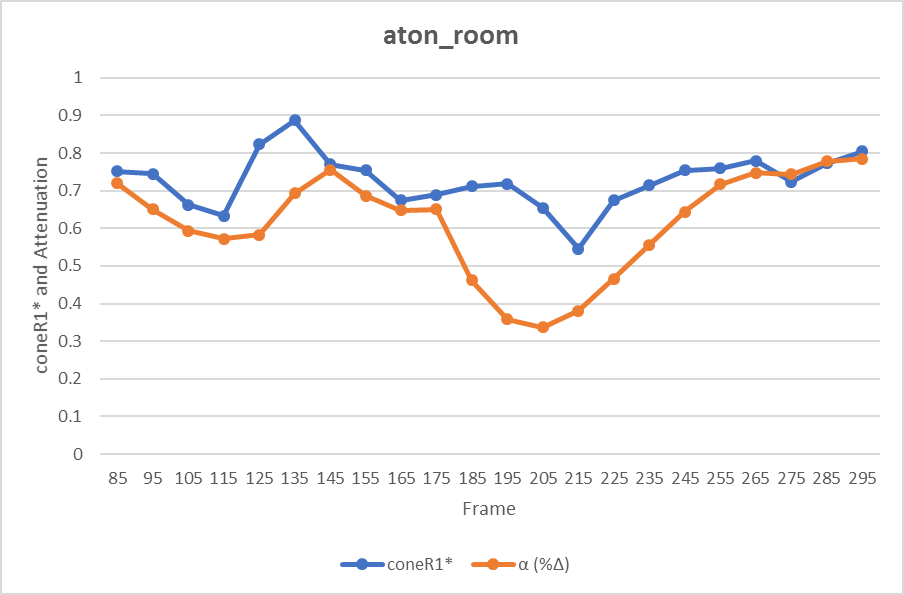
\includegraphics[width=1\linewidth]{figures/appendix/room_rgb.jpg}
  \caption{aton\_room}
\end{subfigure}
\hfill
\begin{subfigure}{.45\linewidth}
  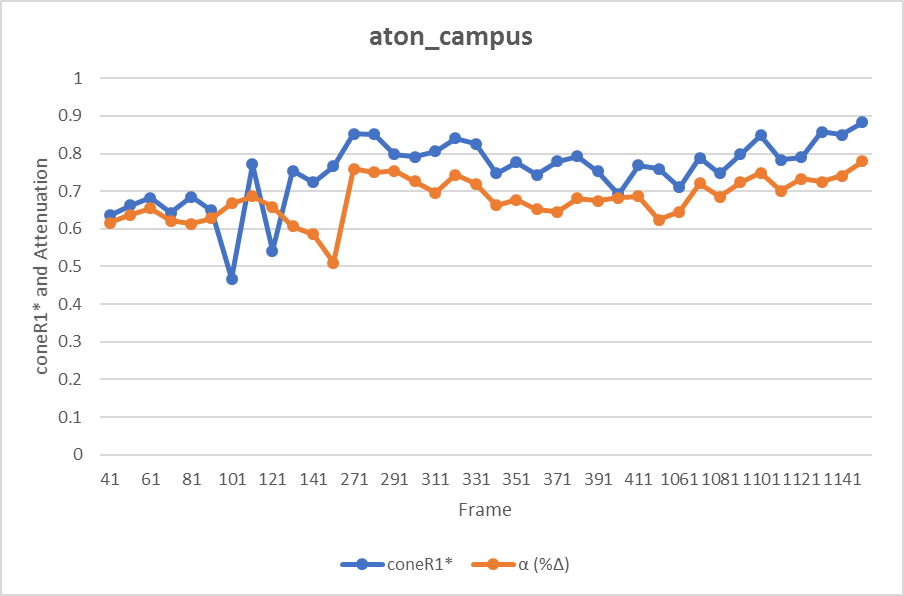
\includegraphics[width=1\linewidth]{figures/appendix/campus_rgb.jpg}
  \caption{aton\_campus}
\end{subfigure}
\hfill
\begin{subfigure}{.45\linewidth}
  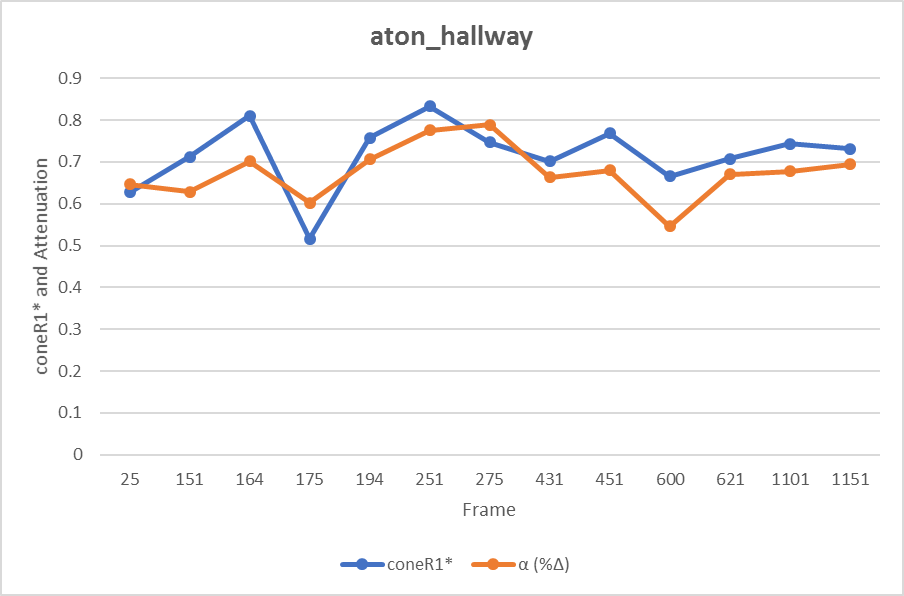
\includegraphics[width=1\linewidth]{figures/appendix/hallway_rgb.jpg}
  \caption{aton\_hallway}
\end{subfigure}
\hfill
\begin{subfigure}{.45\linewidth}
  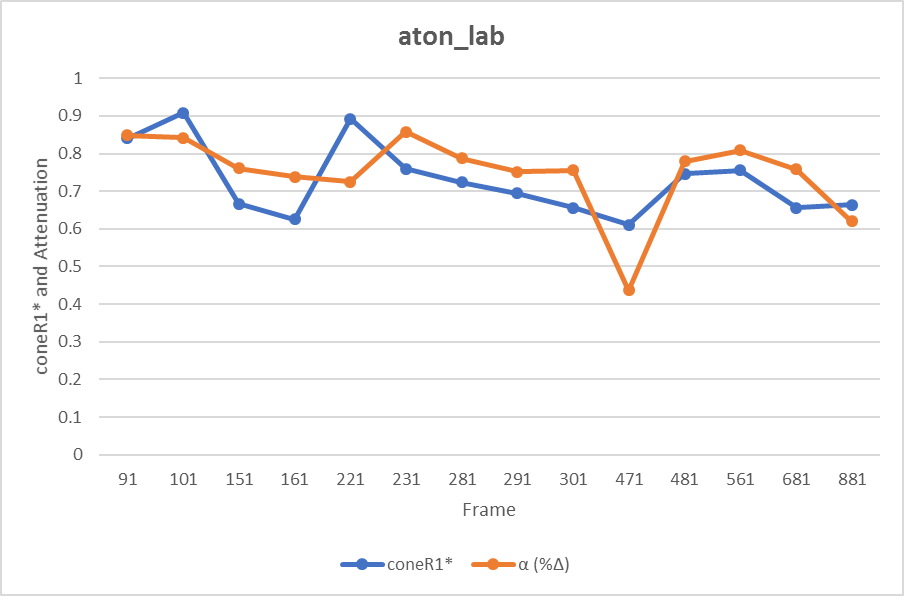
\includegraphics[width=1\linewidth]{figures/appendix/lab_rgb.jpg}
  \caption{aton\_lab}
\end{subfigure}
\caption{Attenuation ($\alpha_{\%\Delta}$ model) plotted against \textit{coneR1}*. (pt. 2 of 2)}

\end{sidewaysfigure}

\clearpage
\FloatBarrier
% SIFT
% 1-4
\begin{sidewaysfigure}

  \begin{subfigure}{.45\linewidth}
  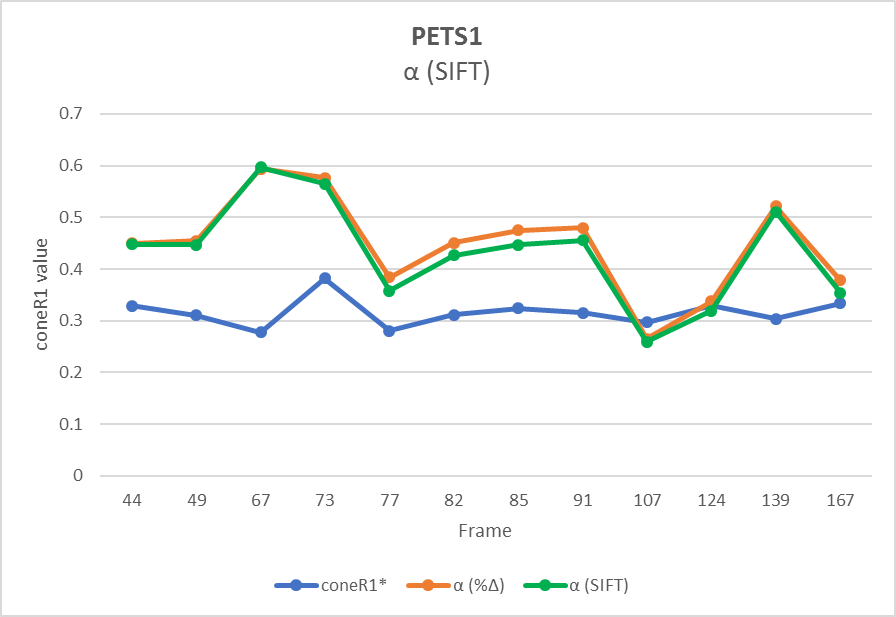
\includegraphics[width=1\linewidth]{figures/appendix/pets1_sift.jpg}
  \caption{PETS1}
\end{subfigure}
\hfill
\begin{subfigure}{.45\linewidth}
  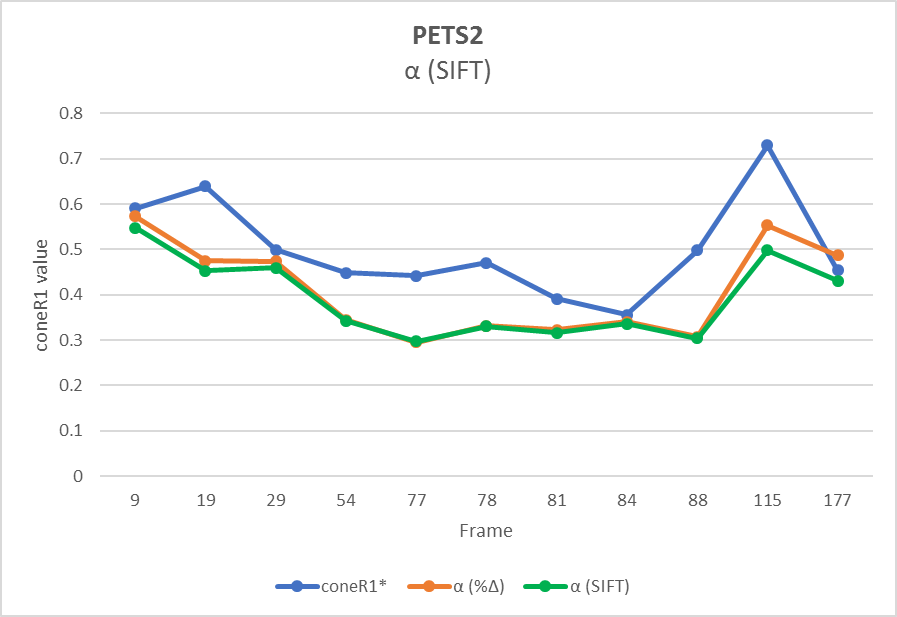
\includegraphics[width=1\linewidth]{figures/appendix/pets2_sift.jpg}
  \caption{PETS2}
\end{subfigure}
\hfill
\begin{subfigure}{.45\linewidth}
  \includegraphics[width=1\linewidth]{figures/appendix/highway1_sift.jpg}
  \caption{aton\_highway1}
\end{subfigure}
\hfill
\begin{subfigure}{.45\linewidth}
  \includegraphics[width=1\linewidth]{figures/appendix/highway3_sift.jpg}
  \caption{aton\_highway3}
\end{subfigure}
\caption{$\alpha_{SIFT}$ (green) is plotted against \textit{coneR1}* and $\alpha_{\%\Delta}$. (pt. 1 of 2)}

\end{sidewaysfigure}

% 5-8
\begin{sidewaysfigure}

  \begin{subfigure}{.45\linewidth}
  \includegraphics[width=1\linewidth]{figures/appendix/room_sift.jpg}
  \caption{aton\_room}
\end{subfigure}
\hfill
\begin{subfigure}{.45\linewidth}
  \includegraphics[width=1\linewidth]{figures/appendix/campus_sift.jpg}
  \caption{aton\_campus}
\end{subfigure}
\hfill
\begin{subfigure}{.45\linewidth}
  \includegraphics[width=1\linewidth]{figures/appendix/hallway_sift.jpg}
  \caption{aton\_hallway}
\end{subfigure}
\hfill
\begin{subfigure}{.45\linewidth}
  \includegraphics[width=1\linewidth]{figures/appendix/lab_sift.jpg}
  \caption{aton\_lab}
\end{subfigure}
\caption{\textit{coneR1}$'$ (green) is plotted against \textit{coneR1}* and $\alpha_{\%\Delta}$. (pt. 2 of 2)}

\end{sidewaysfigure}

\clearpage
\FloatBarrier
% coneR1* & coneR1'
% 1-4
\begin{sidewaysfigure}

  \begin{subfigure}{.45\linewidth}
  \includegraphics[width=1\linewidth]{figures/appendix/pets1_prime.jpg}
  \caption{PETS1}
\end{subfigure}
\hfill
\begin{subfigure}{.45\linewidth}
  \includegraphics[width=1\linewidth]{figures/appendix/pets2_prime.jpg}
  \caption{PETS2}
\end{subfigure}
\hfill
\begin{subfigure}{.45\linewidth}
  \includegraphics[width=1\linewidth]{figures/appendix/highway1_prime.jpg}
  \caption{aton\_highway1}
\end{subfigure}
\hfill
\begin{subfigure}{.45\linewidth}
  \includegraphics[width=1\linewidth]{figures/appendix/highway3_prime.jpg}
  \caption{aton\_highway3}
\end{subfigure}
\caption{$\alpha_{SIFT}$ (green) is plotted against \textit{coneR1}* and $\alpha_{\%\Delta}$. (pt. 1 of 2)}

\end{sidewaysfigure}

% 5-8
\begin{sidewaysfigure}

  \begin{subfigure}{.45\linewidth}
  \includegraphics[width=1\linewidth]{figures/appendix/room_prime.jpg}
  \caption{aton\_room}
\end{subfigure}
\hfill
\begin{subfigure}{.45\linewidth}
  \includegraphics[width=1\linewidth]{figures/appendix/campus_prime.jpg}
  \caption{aton\_campus}
\end{subfigure}
\hfill
\begin{subfigure}{.45\linewidth}
  \includegraphics[width=1\linewidth]{figures/appendix/hallway_prime.jpg}
  \caption{aton\_hallway}
\end{subfigure}
\hfill
\begin{subfigure}{.45\linewidth}
  \includegraphics[width=1\linewidth]{figures/appendix/lab_prime.jpg}
  \caption{aton\_lab}
\end{subfigure}
\caption{\textit{coneR1}$'$ (green) is plotted against \textit{coneR1}* and $\alpha_{\%\Delta}$. (pt. 2 of 2)}

\end{sidewaysfigure}

% New Detection and Discrimination
% PETS1
\begin{table}
\centering
\caption{PETS1 - Detection and Discrimination rates calculated for both default coneR1 (Original) and coneR1$'$ (Adaptive).}
%\caption*{Detection and Discrimination rates calculated for both default coneR1 (Original) and coneR1$'$ (Adaptive).}
\begin{tabular}{ |c|c|c|c|c|c|c| }
\hline
\textbf{frame} &  \textbf{coneR1*} &  \textbf{coneR1$'$} &  \textbf{Original $\eta$} &  \textbf{Adaptive $\eta$} &  \textbf{Original $\xi$} &  \textbf{Adaptive $\xi$} \\
\hline
\hline
44 &  0.329 &  0.223804 &  69.2827 &  69.9578 &  75.9517 &  73.8973 \\
\hline
49 &  0.31 &  0.246728 &  53.108 &  53.6512 &  83.4889 &  81.4617 \\
\hline
67 &  0.278 &  0.402792 &  65.6433 &  58.9181 &  67.6909 &  71.1704 \\
\hline
73 &  0.382 &  0.393097 &  66.2295 &  63.9344 &  64.7059 &  68.0561 \\
\hline
77 &  0.28 &  0.192245 &  79.6947 &  82.1374 &  76.039 &  72.5529 \\
\hline
82 &  0.311 &  0.222533 &  78.6989 &  80.3717 &  73.8816 &  69.7234 \\
\hline
85 &  0.324 &  0.265211 &  68.8791 &  69.5225 &  66.9706 &  64.903 \\
\hline
91 &  0.315 &  0.288086 &  71.5467 &  72.0817 &  68.4584 &  68.0297 \\
\hline
107 &  0.297 &  0.0550418 &  63.1347 &  64.4592 &  80.6748 &  71.3574 \\
\hline
124 &  0.329 &  0.117233 &  79.3729 &  86.3036 &  66.0321 &  47.3447 \\
\hline
139 &  0.304 &  0.324891 &  89.7321 &  88.8393 &  57.1618 &  57.4271 \\
\hline
167 &  0.334 &  0.173734 &  88.5057 &  89.1626 &  80.3523 &  77.3713 \\
\hline
\end{tabular}

\end{table}
% New Detection and Discrimination
% PETS2
\begin{table}
\centering
\caption{PETS2 - Detection and Discrimination rates calculated for both default coneR1 (Original) and coneR1$'$ (Adaptive).}
%\caption*{Detection and Discrimination rates calculated for both default coneR1 (Original) and coneR1$'$ (Adaptive).}
\begin{tabular}{ |c|c|c|c|c|c|c| }
\hline
\textbf{frame} &  \textbf{coneR1*} &  \textbf{coneR1$'$} &  \textbf{Original $\eta$} &  \textbf{Adaptive $\eta$} &  \textbf{Original $\xi$} &  \textbf{Adaptive $\xi$} \\
\hline
\hline
9 &  0.591 &  0.392866 &  68.0879 &  68.0879 &  76.4585 &  78.5824 \\
\hline
19 &  0.639 &  0.277102 &  33.5938 &  33.5938 &  84.7328 &  84.2682 \\
\hline
29 &  0.499 &  0.251038 &  33.9921 &  33.9921 &  84.0453 &  83.1735 \\
\hline
54 &  0.448 &  0.102197 &  99.115 &  99.115 &  66.7976 &  31.0413 \\
\hline
77 &  0.442 &  0.0969234 &  99.2218 &  99.2218 &  70.5216 &  57.3393 \\
\hline
78 &  0.471 &  0.129563 &  100 &  100 &  66.2837 &  49.4034 \\
\hline
81 &  0.391 &  0.147082 &  96.9161 &  97.1689 &  76.2933 &  70.1039 \\
\hline
84 &  0.356 &  0.157141 &  92.2688 &  92.6301 &  74.164 &  69.3635 \\
\hline
88 &  0.498 &  0.11751 &  100 &  100 &  62.7468 &  43.525 \\
\hline
115 &  0.73 &  0.374374 &  20.2454 &  20.2454 &  65.5239 &  67.8525 \\
\hline
177 &  0.454 &  0.298634 &  73.6506 &  73.6506 &  69.8562 &  69.7363 \\

\hline
\end{tabular}

\end{table}

% New Detection and Discrimination
% aton_highway1
\begin{table}
\centering
\caption{aton\_highway1 - Detection and Discrimination rates calculated for both default coneR1 (Original) and coneR1$'$ (Adaptive).}
%\caption*{Detection and Discrimination rates calculated for both default coneR1 (Original) and coneR1$'$ (Adaptive).}
\begin{tabular}{ |c|c|c|c|c|c|c| }
\hline
\textbf{frame} &  \textbf{coneR1*} &  \textbf{coneR1$'$} &  \textbf{Original $\eta$} &  \textbf{Adaptive $\eta$} &  \textbf{Original $\xi$} &  \textbf{Adaptive $\xi$} \\
\hline
\hline
45 &  0.233 &  0.220497 &  75.55 &  87.2782 &  69.2299 &  61.9624 \\
\hline
65 &  0.311 &  0.220315 &  67.158 &  72.2248 &  65.4284 &  52.7443 \\
\hline
85 &  0.214 &  0.216213 &  73.1796 &  84.2697 &  58.4456 &  51.8659 \\
\hline
105 &  0.265 &  0.209683 &  82.7473 &  88.022 &  69.9272 &  62.7913 \\
\hline
125 &  0.258 &  0.233547 &  69.1618 &  81.1887 &  63.6085 &  54.9916 \\
\hline
145 &  0.275 &  0.219385 &  72.2989 &  80.6568 &  64.8861 &  56.0676 \\
\hline
165 &  0.249 &  0.223016 &  67.2983 &  77.5194 &  63.1035 &  55.607 \\
\hline
185 &  0.24 &  0.229775 &  65.7503 &  76.8051 &  67.1285 &  60.3536 \\
\hline
\end{tabular}

\end{table}

% New Detection and Discrimination
% aton_highway3
\begin{table}
\centering
\caption{aton\_highway3 - Detection and Discrimination rates calculated for both default coneR1 (Original) and coneR1$'$ (Adaptive).}
%\caption*{Detection and Discrimination rates calculated for both default coneR1 (Original) and coneR1$'$ (Adaptive).}
\begin{tabular}{ |c|c|c|c|c|c|c| }
\hline
\textbf{frame} &  \textbf{coneR1*} &  \textbf{coneR1$'$} &  \textbf{Original $\eta$} &  \textbf{Adaptive $\eta$} &  \textbf{Original $\xi$} &  \textbf{Adaptive $\xi$} \\
\hline
101 &  0.468 &  0.387717 &  75.625 &  75.625 &  35.123 &  37.1365 \\
\hline
201 &  0.325 &  0.394711 &  71.6456 &  67.3418 &  37.7417 &  39.9072 \\
\hline
301 &  0.465 &  0.44571 &  72.1311 &  70.9016 &  45.23 &  50.0852 \\
\hline
501 &  0.37 &  0.276136 &  73.5925 &  73.5925 &  67.1176 &  67.1176 \\
\hline
601 &  0.745 &  0.476506 &  85.1695 &  82.6271 &  36.7862 &  45.6839 \\
\hline
801 &  0.361 &  0.277987 &  74.0392 &  74.0392 &  34.5425 &  34.1364 \\
\hline
1401 &  0.73 &  0.530566 &  80 &  80 &  41.2587 &  50.3497 \\
\hline

\end{tabular}

\end{table}

% New Detection and Discrimination
% aton_room
\begin{table}
\centering
\caption{aton\_room - Detection and Discrimination rates calculated for both default coneR1 (Original) and coneR1$'$ (Adaptive).}
%\caption*{Detection and Discrimination rates calculated for both default coneR1 (Original) and coneR1$'$ (Adaptive).}
\begin{tabular}{ |c|c|c|c|c|c|c| }
\hline
\textbf{frame} &  \textbf{coneR1*} &  \textbf{coneR1$'$} &  \textbf{Original $\eta$} &  \textbf{Adaptive $\eta$} &  \textbf{Original $\xi$} &  \textbf{Adaptive $\xi$} \\
\hline
\hline
85 &  0.751 &  0.649083 &  98.3146 &  97.191 &  40.4321 &  71.6049 \\
\hline
95 &  0.745 &  0.484626 &  96.2506 &  95.8559 &  65.4899 &  80.2594 \\
\hline
105 &  0.662 &  0.377712 &  91.674 &  91.054 &  74.0519 &  82.3353 \\
\hline
115 &  0.634 &  0.30766 &  93.0137 &  93.0137 &  82.6196 &  82.8715 \\
\hline
125 &  0.824 &  0.328275 &  89.6272 &  89.6272 &  78.0451 &  80.3008 \\
\hline
135 &  0.887 &  0.483102 &  96.3006 &  95.6069 &  64.1892 &  78.5473 \\
\hline
145 &  0.77 &  0.558232 &  96.7391 &  96.0474 &  65.8031 &  78.7565 \\
\hline
155 &  0.754 &  0.443622 &  94.9045 &  94.6921 &  73.3198 &  80.8554 \\
\hline
165 &  0.674 &  0.391485 &  93.8378 &  93.2973 &  69.0015 &  74.0686 \\
\hline
175 &  0.689 &  0.397271 &  93.6877 &  93.3555 &  70.3377 &  75.7709 \\
\hline
185 &  0.712 &  0.147542 &  82.381 &  83.3333 &  73.8574 &  57.7697 \\
\hline
195 &  0.719 &  0.0423129 &  61.1111 &  64.8148 &  70.6796 &  34.3689 \\
\hline
205 &  0.655 &  0.0391442 &  54.8387 &  54.8387 &  70.8333 &  42.6136 \\
\hline
215 &  0.545 &  0.105035 &  48.913 &  50 &  70.3166 &  49.2084 \\
\hline
225 &  0.674 &  0.20744 &  86.25 &  86.5625 &  63.7487 &  54.6859 \\
\hline
235 &  0.715 &  0.337354 &  95.037 &  94.9314 &  73.5849 &  75.5503 \\
\hline
245 &  0.754 &  0.492393 &  97.561 &  97.1458 &  65.1096 &  77.624 \\
\hline
255 &  0.759 &  0.627669 &  99.0716 &  98.6822 &  65.9314 &  85.6863 \\
\hline
265 &  0.779 &  0.687616 &  99.2512 &  97.6628 &  62.6719 &  85.8939 \\
\hline
275 &  0.724 &  0.655212 &  98.8365 &  97.5761 &  66.711 &  89.0957 \\
\hline
285 &  0.773 &  0.733917 &  99.4827 &  98.3026 &  68.1431 &  90.2896 \\
\hline
295 &  0.805 &  0.709282 &  99.0119 &  96.6984 &  62.855 &  85.6879 \\
\hline
\end{tabular}

\end{table}

% New Detection and Discrimination
% aton_campus
\begin{table}
\centering
\caption{aton\_campus - Detection and Discrimination rates calculated for both default coneR1 (Original) and coneR1$'$ (Adaptive).}
%\caption*{Detection and Discrimination rates calculated for both default coneR1 (Original) and coneR1$'$ (Adaptive).}
\begin{tabular}{ |c|c|c|c|c|c|c| }
\hline
\textbf{frame} &  \textbf{coneR1*} &  \textbf{coneR1$'$} &  \textbf{Original $\eta$} &  \textbf{Adaptive $\eta$} &  \textbf{Original $\xi$} &  \textbf{Adaptive $\xi$} \\
\hline
\hline
41 &  0.636 &  0.434367 &  100 &  100 &  2.139 &  17.9144 \\
\hline
51 &  0.662 &  0.469132 &  99.9291 &  99.5272 &  11.5192 &  33.9065 \\
\hline
61 &  0.683 &  0.495272 &  99.9034 &  95.9259 &  31.9713 &  59.868 \\
\hline
71 &  0.642 &  0.454936 &  99.0625 &  93.3413 &  32.0908 &  54.5861 \\
\hline
81 &  0.685 &  0.444833 &  96.8359 &  91.9249 &  29.5123 &  46.1152 \\
\hline
91 &  0.649 &  0.466827 &  98.3946 &  94.7157 &  36.9529 &  51.9231 \\
\hline
101 &  0.467 &  0.522102 &  100 &  93.3692 &  44.0171 &  55.6058 \\
\hline
111 &  0.772 &  0.552027 &  97.0534 &  97.0534 &  58.1594 &  67.0103 \\
\hline
121 &  0.542 &  0.514771 &  97.4386 &  91.1419 &  38.9846 &  55.8306 \\
\hline
131 &  0.754 &  0.448236 &  96.8276 &  92.6897 &  32.298 &  46.3734 \\
\hline
141 &  0.724 &  0.426879 &  90.6977 &  90.6977 &  52.2929 &  70.858 \\
\hline
151 &  0.766 &  0.301711 &  72.8814 &  72.8814 &  38.3412 &  38.5308 \\
\hline
271 &  0.852 &  0.671848 &  100 &  100 &  49.2236 &  78.5714 \\
\hline
281 &  0.851 &  0.656997 &  100 &  100 &  40.597 &  73.8308 \\
\hline
291 &  0.798 &  0.659748 &  100 &  100 &  39.1304 &  70.5828 \\
\hline
301 &  0.791 &  0.616497 &  99.4709 &  99.4709 &  44.2506 &  72.7201 \\
\hline
311 &  0.806 &  0.572523 &  100 &  100 &  41.1673 &  64.0467 \\
\hline
321 &  0.84 &  0.649439 &  100 &  100 &  40.3864 &  73.5051 \\
\hline
331 &  0.826 &  0.612811 &  100 &  100 &  28.903 &  64.346 \\
\hline
341 &  0.748 &  0.53507 &  99.3392 &  99.3392 &  21.3919 &  53.3942 \\
\hline
351 &  0.777 &  0.559359 &  99.3342 &  98.8016 &  16.0519 &  57.8182 \\
\hline
361 &  0.743 &  0.521477 &  99.729 &  99.729 &  18.6912 &  47.6871 \\
\hline
371 &  0.779 &  0.508699 &  95.6188 &  95.6188 &  13.4861 &  44.0589 \\
\hline
381 &  0.793 &  0.545052 &  99.3644 &  99.3644 &  20.6265 &  69.3247 \\
\hline
391 &  0.753 &  0.534082 &  92.4701 &  92.3997 &  21.9302 &  64.9692 \\
\hline
401 &  0.692 &  0.541953 &  94.5976 &  94.4851 &  22.5201 &  73.4201 \\
\hline
411 &  0.769 &  0.541069 &  92.452 &  92.452 &  23.6516 &  75 \\
\hline
421 &  0.759 &  0.450694 &  92.1158 &  92.1158 &  25.9178 &  61.674 \\
\hline
1061 &  0.711 &  0.515943 &  100 &  100 &  14.4099 &  40.6211 \\
\hline
1071 &  0.789 &  0.636891 &  100 &  100 &  15.9018 &  50.4803 \\
\hline
1081 &  0.748 &  0.583271 &  100 &  100 &  28.5558 &  49.2341 \\
\hline
1091 &  0.798 &  0.628366 &  98.2456 &  98.2456 &  24.4784 &  48.1224 \\
\hline
1101 &  0.848 &  0.65963 &  100 &  100 &  10.1961 &  46.6667 \\
\hline
1111 &  0.784 &  0.586309 &  96.2025 &  95.5696 &  12.0468 &  52.6316 \\
\hline
1121 &  0.79 &  0.631131 &  98.75 &  98.75 &  17.64 &  56.7342 \\
\hline
1131 &  0.858 &  0.616672 &  97.9167 &  97.9167 &  18.595 &  58.6777 \\
\hline
1141 &  0.85 &  0.63811 &  98.3871 &  98.3871 &  15.9574 &  63.2388 \\
\hline
1151 &  0.883 &  0.700727 &  99.4723 &  99.4723 &  6.2691 &  57.9511 \\
\hline
\end{tabular}

\end{table}

% New Detection and Discrimination
% aton_hallway
\begin{table}
\centering
\caption{aton\_hallway - Detection and Discrimination rates calculated for both default coneR1 (Original) and coneR1$'$ (Adaptive).}
%\caption*{Detection and Discrimination rates calculated for both default coneR1 (Original) and coneR1$'$ (Adaptive).}
\begin{tabular}{ |c|c|c|c|c|c|c| }
\hline
\textbf{frame} &  \textbf{coneR1*} &  \textbf{coneR1$'$} &  \textbf{Original $\eta$} &  \textbf{Adaptive $\eta$} &  \textbf{Original $\xi$} &  \textbf{Adaptive $\xi$} \\
\hline
\hline
25 &  0.627 &  0.459744 &  91.8856 &  91.4769 &  64.1346 &  74.6609 \\
\hline
151 &  0.712 &  0.434228 &  99.6218 &  99.5083 &  69.3347 &  78.6133 \\
\hline
164 &  0.81 &  0.538867 &  97.5408 &  97.4856 &  55.5124 &  71.1619 \\
\hline
175 &  0.516 &  0.391069 &  87.1708 &  82.9169 &  63.6149 &  67.8378 \\
\hline
194 &  0.758 &  0.586353 &  99.3337 &  99.2945 &  76.1484 &  83.7938 \\
\hline
251 &  0.833 &  0.664601 &  82.2111 &  81.3065 &  81.7981 &  86.5144 \\
\hline
275 &  0.747 &  0.690587 &  98.7539 &  97.5078 &  78.8321 &  88.0779 \\
\hline
431 &  0.702 &  0.471719 &  99.407 &  99.2453 &  59.2399 &  67.6975 \\
\hline
451 &  0.769 &  0.54227 &  99.3588 &  99.2145 &  80.6987 &  86.1682 \\
\hline
600 &  0.666 &  0.379226 &  63.4615 &  63.4615 &  73.7265 &  75.067 \\
\hline
621 &  0.707 &  0.478939 &  99.6299 &  98.9309 &  48.4927 &  60.5728 \\
\hline
1101 &  0.743 &  0.48757 &  98.4813 &  98.4343 &  83.9228 &  89.4248 \\
\hline
1151 &  0.731 &  0.554371 &  99.572 &  99.0661 &  83.2968 &  87.2946 \\
\hline
\end{tabular}

\end{table}

% New Detection and Discrimination
% aton_lab
\begin{table}
\centering
\caption{aton\_lab - Detection and Discrimination rates calculated for both default coneR1 (Original) and coneR1$'$ (Adaptive).}
%\caption*{Detection and Discrimination rates calculated for both default coneR1 (Original) and coneR1$'$ (Adaptive).}
\begin{tabular}{ |c|c|c|c|c|c|c| }
\hline
\textbf{frame} &  \textbf{coneR1*} &  \textbf{coneR1$'$} &  \textbf{Original $\eta$} &  \textbf{Adaptive $\eta$} &  \textbf{Original $\xi$} &  \textbf{Adaptive $\xi$} \\
\hline
\hline
91 &  0.84 &  0.747661 &  98.2784 &  96.1688 &  44.6844 &  64.6179 \\
\hline
101 &  0.908 &  0.729663 &  97.5334 &  97.5107 &  39.4961 &  63.1496 \\
\hline
151 &  0.667 &  0.573093 &  95.804 &  95.4925 &  82.9254 &  93.3515 \\
\hline
161 &  0.626 &  0.540102 &  93.4618 &  93.1693 &  80.3861 &  89.7572 \\
\hline
221 &  0.892 &  0.509917 &  87.9733 &  87.9733 &  66.7318 &  70.371 \\
\hline
231 &  0.76 &  0.771263 &  95.973 &  94.2403 &  61.1534 &  81.9075 \\
\hline
281 &  0.724 &  0.629486 &  94.8925 &  94.1761 &  79.6353 &  90.1867 \\
\hline
291 &  0.695 &  0.555757 &  97.0733 &  97.0551 &  77.8626 &  92.2074 \\
\hline
301 &  0.656 &  0.561814 &  88.5236 &  88.3742 &  85.6973 &  96.1859 \\
\hline
471 &  0.611 &  0.129561 &  78.898 &  90.1524 &  83.0598 &  58.7802 \\
\hline
481 &  0.746 &  0.615002 &  97.2113 &  96.9035 &  76.6697 &  86.9145 \\
\hline
561 &  0.755 &  0.670057 &  97.4796 &  96.0158 &  60.1613 &  74.2868 \\
\hline
681 &  0.656 &  0.589291 &  95.7642 &  94.3217 &  62.9807 &  75.444 \\
\hline
881 &  0.664 &  0.350949 &  82.1207 &  82.1207 &  83.7588 &  85.0625 \\
\hline
\end{tabular}

\end{table}

\end{appendices}